\documentclass[12pt]{article}
\pdfoutput=1
\setlength{\oddsidemargin}{0in}
\setlength{\evensidemargin}{0in}
\setlength{\textwidth}{6.5in}
\setlength{\topmargin}{-.25in}
\setlength{\headheight}{0in}
\setlength{\textheight}{9in}

\newcommand{\globes}{\sf{GLoBES}}
\newcommand{\snowglobes}{\sf{SNOwGLoBES}}
\usepackage{graphicx}
\usepackage{url}
\begin{document}

\title{\bf $\snowglobes$: SuperNova Observatories with $\globes$: DRAFT}
\author{Joshua Albert$^1$,
Alex Beck$^1$,
Farzan Beroz$^1$,
Rachel Carr$^2$,
Huaiyu Duan$^3$,\\
Alex Friedland$^4$,
Nicolas Kaiser$^{5,1}$,
Jim Kneller$^6$,
Alexander Moss$^1$,\\
Diane Reitzner$^7$,
Kate Scholberg$^{1*}$,
David Webber$^8$,
Roger Wendell$^1$\\
~\\
\small
$^1$ Department of Physics, Duke University, Durham, NC 27705\\
\small
$^2$ Department of Physics, Columbia University, New York, NY 10027\\
\small
$^3$ Department of Physics, University of New Mexico, Albuquerque, NM, 87131\\
\small
$^4$ Los Alamos National Laboratory, Los Alamos, NM, 87545\\
\small
$^5$ Department of Physics, Karlsruhe Institute of Technology, Germany\\
\small
$^6$ Department of Physics, North Carolina State University, Raleigh, NC,  27695\\
\small
$^7$ Fermilab, Batavia, IL, 60510-5011\\
\small
$^8$ Department of Physics, University of Wisconsin, Madison, WI, 53706-1390\\
\small
$^*$ \texttt{schol@phy.duke.edu}\\
}

\date{Version 1.1 \today}

\maketitle 


\begin{abstract} 
This document describes public software
  for computing interaction rates and distributions of observed
  quantities for supernova burst neutrinos in common detector
  materials.  The intent is to provide a very simple and fast 
  code and data
  package which
  can be used for tests of observability of physics signatures in
  current and future detectors, and for evaluation of relative
  sensitivities of different detector configurations.  The event
  estimates are made using available cross-sections and
  parameterized detector responses.  Water, argon, scintillator
  and lead-based configurations are included.
  The package makes use of $\globes$
  front-end software.  $\snowglobes$ is not intended to replace full
  detector simulations; however output should be useful for many types
  of studies.  This document serves as a user's manual and provides 
  references for the data files used.

\end{abstract}

\section{Introduction}

A stellar core collapse in the Milky Way or nearby will produce an enormous burst of neutrinos observable in terrestrial detectors.  Such a burst will carry tremendous information about both astrophysics and particle physics: see~\cite{Dighe:2008dq} for recent reviews of physics reach and ~\cite{Scholberg:2007nu} for an overview of detection technology.

To enable fast, informative studies of the physics potential of the
detection of supernova neutrinos, we have developed a simple software
and database package to compute expected event rates by folding input
fluxes with cross-sections and detector  parameters.  The output is in the
form of interaction rates for each channel as a function of neutrino
energy, and ``smeared'' rates as a function of detected energy for
each channel (\textit{i.e.} the spectrum that actually be observed in a
detector).  For this study we have chosen to do the event rate
computation by using parameterized detector responses, making use of
the $\globes$ software~\cite{Huber:2004ka,globes}.  We employ only the front-end rate
engine part of $\globes$, and not the oscillation sensitivity part.
$\globes$ takes as input fluxes, cross sections, ``smearing matrices''
and post-smearing efficiencies.  The smearing matrices incorporate
both interaction product spectra and detector response.
Fig.~\ref{fig:schematic} gives a schematic overview of the approach.

\begin{figure}
\begin{center}
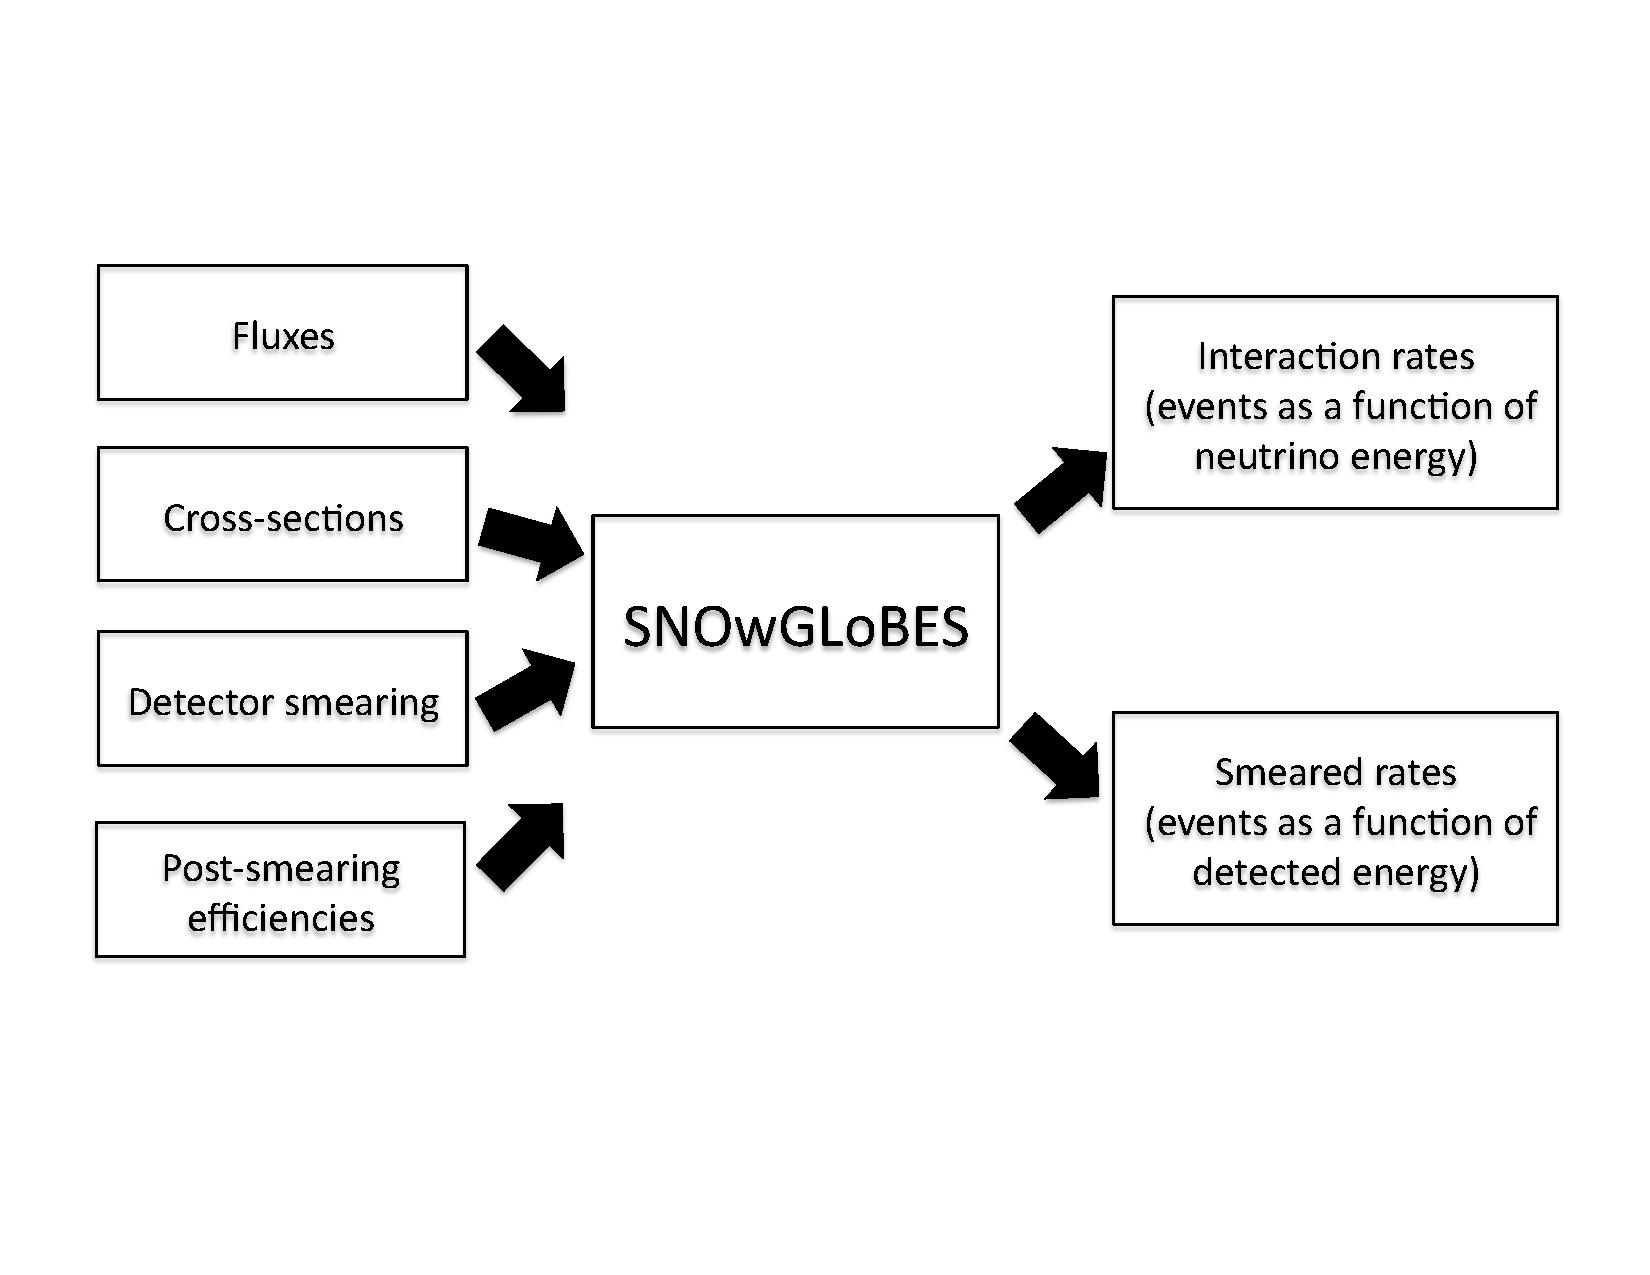
\includegraphics[height=.3\textheight]{figures/schematic.pdf}
\end{center}
\caption{$\snowglobes$ data flow.}\label{fig:schematic}
\end{figure}



Although with this approach, information is lost with respect to a
full event-by-event simulation using a neutrino interaction generator
and detector simulation (correlations between energy and angle are
lost, for example), nevertheless it offers a fast, simple method
useful for many studies.

The software should enable studies from differing points of view, by
allowing modification of the different kinds of input.  For example:

\begin{itemize}

\item Using the standard cross-sections and detector parameters, one
  can study whether specific physics signatures in the fluxes are observable
  with different detector configurations.

\item Experimentalists can optimize detector configurations by using
  standard cross-sections and the sample fluxes, and modifying the
  smearing, efficiency and background files according to different configurations
  (for example, different PMT coverages in a water Cherenkov configuration).  An early version of $\snowglobes$ was used in this way for the work described in reference~\cite{pwgstudy}.

\item 
One could also study systematic errors due to cross-section
uncertainties (for example) by comparing event rates computed using cross-sections
from different models or with modifications according to estimated
uncertainties.

\end{itemize}

Currently, time-dependent fluxes are not supported explicitly; however
time dependence can be straightforwardly handled by providing multiple
files with fluxes divided into different time bins.

Users should note that \textit{$\snowglobes$ does not employ the oscillation probability and parameter sensitivity computation functionality of $\globes$ at all}.  Although $\snowglobes$ can be helpful for studies of neutrino oscillation by, for example, enabling the comparison of expected  oscillated and non-oscillated fluxes (for oscillation in supernova or Earth), the user must compute the oscillation probabilities modulating the flux and evaluate sensitivities separately.
$\snowglobes$ is simply an event rate calculator.

\section{Software Overview}

\subsection{Dependencies}

$\globes$~\cite{globes} version 3.0.15 or later and its dependencies
(3.1.6 for Mac)  must be installed, and the
environment variable \texttt{GLB\_DIR} must be set to the $\globes$
installation directory.  \texttt{Perl} is also required, and \texttt{Root}~\cite{root} is required for the sample plotting scripts.

\subsection{Download and Installation Instructions}

The package is available from the Duke \texttt{svn} repository.

\begin{itemize}
\item Download version 1.1 with

\noindent
\texttt{svn co http://svn.phy.duke.edu/repos/neutrino/snowglobes/tags/snowglobes-1.1}

with userid and password \texttt{guest/guest}.

\item Set the environment variable \texttt{SNOWGLOBES} to the installation directory.  

\item Set the environment variable \texttt{GLB\_DIR} to where you have installed $\globes$.

\item Go to \texttt{\$SNOWGLOBES/src} and type \texttt{make}, then
\texttt{make install}.  

\item That's it.  Run the scripts from the \texttt{\$SNOWGLOBES} directory.

\end{itemize}

\subsection{Files}

The $\snowglobes$ package has data files organized into several subdirectories:

\begin{itemize}

\item \texttt{\$SNOWGLOBES/backgrounds}  contains the additive background files, labeled by detector configuration. 


\item \texttt{\$SNOWGLOBES/bin}  contains the $\globes$ executable run by the main script.

\item \texttt{\$SNOWGLOBES/channels}  contains the
files listing relevant channels for each detector type.

\item \texttt{\$SNOWGLOBES/doc}  contains documentation for installation and running, and references for the included data files.


\item \texttt{\$SNOWGLOBES/effic}  contains the
 post-smearing efficiency files in $\globes$ format, labeled by interaction type and detector configuration.

\item \texttt{\$SNOWGLOBES/fluxes}  contains the flux files in $\globes$ format, labeled by flux name.

\item \texttt{\$SNOWGLOBES/glb}  contains some template files required for building the $\globes$ file.

\item \texttt{\$SNOWGLOBES/out} contains output files generated by
  $\snowglobes$, labeled by interaction type and detector configuration,
  for both interaction rates and smeared rates.   

\item \texttt{\$SNOWGLOBES/plots} contains some sample Root plotting scripts.

\item \texttt{\$SNOWGLOBES/smear}  contains the smearing matrix files in $\globes$ format, labeled by interaction type and detector configuration.

\item \texttt{\$SNOWGLOBES/xscns}  contains the cross-section files in $\globes$ format, labeled by interaction channel.



\end{itemize}


\subsection{Running the Software}

The primary tool is a script called \texttt{supernova.pl}.  This takes three arguments: the flux file label, the channel file label, and the experiment configuration name.

The channel file gives a list of channels for which $\snowglobes$
should compute event rates, and the appropriate target weighting
factor for each of these channels.  Example channels files can be
found in the \texttt{\$SNOWGLOBES/channels} subdirectory.  The user can
modify these to select desired channels.  See section~\ref{addingnew}
for information about how to add new channels.

For example, to compute event rates for HALO2 for ``Livermore'' flux and  the interaction channels in
\texttt{\$SNOWGLOBES/channels/channels\_lead.dat}, do\\

\texttt{./supernova.pl livermore lead halo2} \\

Output goes to the \texttt{\$SNOWGLOBES/out} subdirectory, into spectrum files
named by flux, channel, and experiment configuration.  Output text
files are generated both for interaction rates (as a function of
neutrino energy), and for rates smeared by detector response, as a
function of detected energy (the latter are labeled ``\texttt{\_smeared}'').  The
first column of the output file is energy (either neutrino energy or,
for smeared output, detected energy), and the second column is event
rate in that energy bin (events per 0.5 MeV).

Files for which event rates are not weighted by target weighting factor (see section~\ref{addingchannel}) are labeled ``\texttt{\_unweighted}''.  As of 
$\snowglobes$ version 1.1, the \texttt{supernova.pl} script applies the weighting factors to create the output files.

\texttt{make\_event\_table.pl} is a sample script to return integrated
rates for each channel.   It takes the same arguments as \texttt{supernova.pl}; add an additional argument ``1'' if a table of non-smeared rates is desired.
The
plotting scripts in the \texttt{\$SNOWGLOBES/plots} directory also
give examples of plotting output rates. 

\section{Supernova Neutrino Fluxes}

Supernova neutrino fluxes must be provided in $\globes$ file format.  Two
example fluxes are provided with the package: the ``Livermore''
flux~\cite{Totani:1997vj}, and the ``GKVM'' flux~\cite{Gava:2009pj}.
Strictly speaking, these are not fluxes but fluences: they are
integrated over the time of the burst.  The spectra for the flavor
components of these two example fluences are plotted in
Fig.~\ref{fig:fluxes}.  We will include more fluxes, and flux generation tools, in the future.

% Add this later
%Also provided is some C++ software that will produce ``pinched''
%spectra for specified values of $\alpha$ and temperature

\begin{figure}
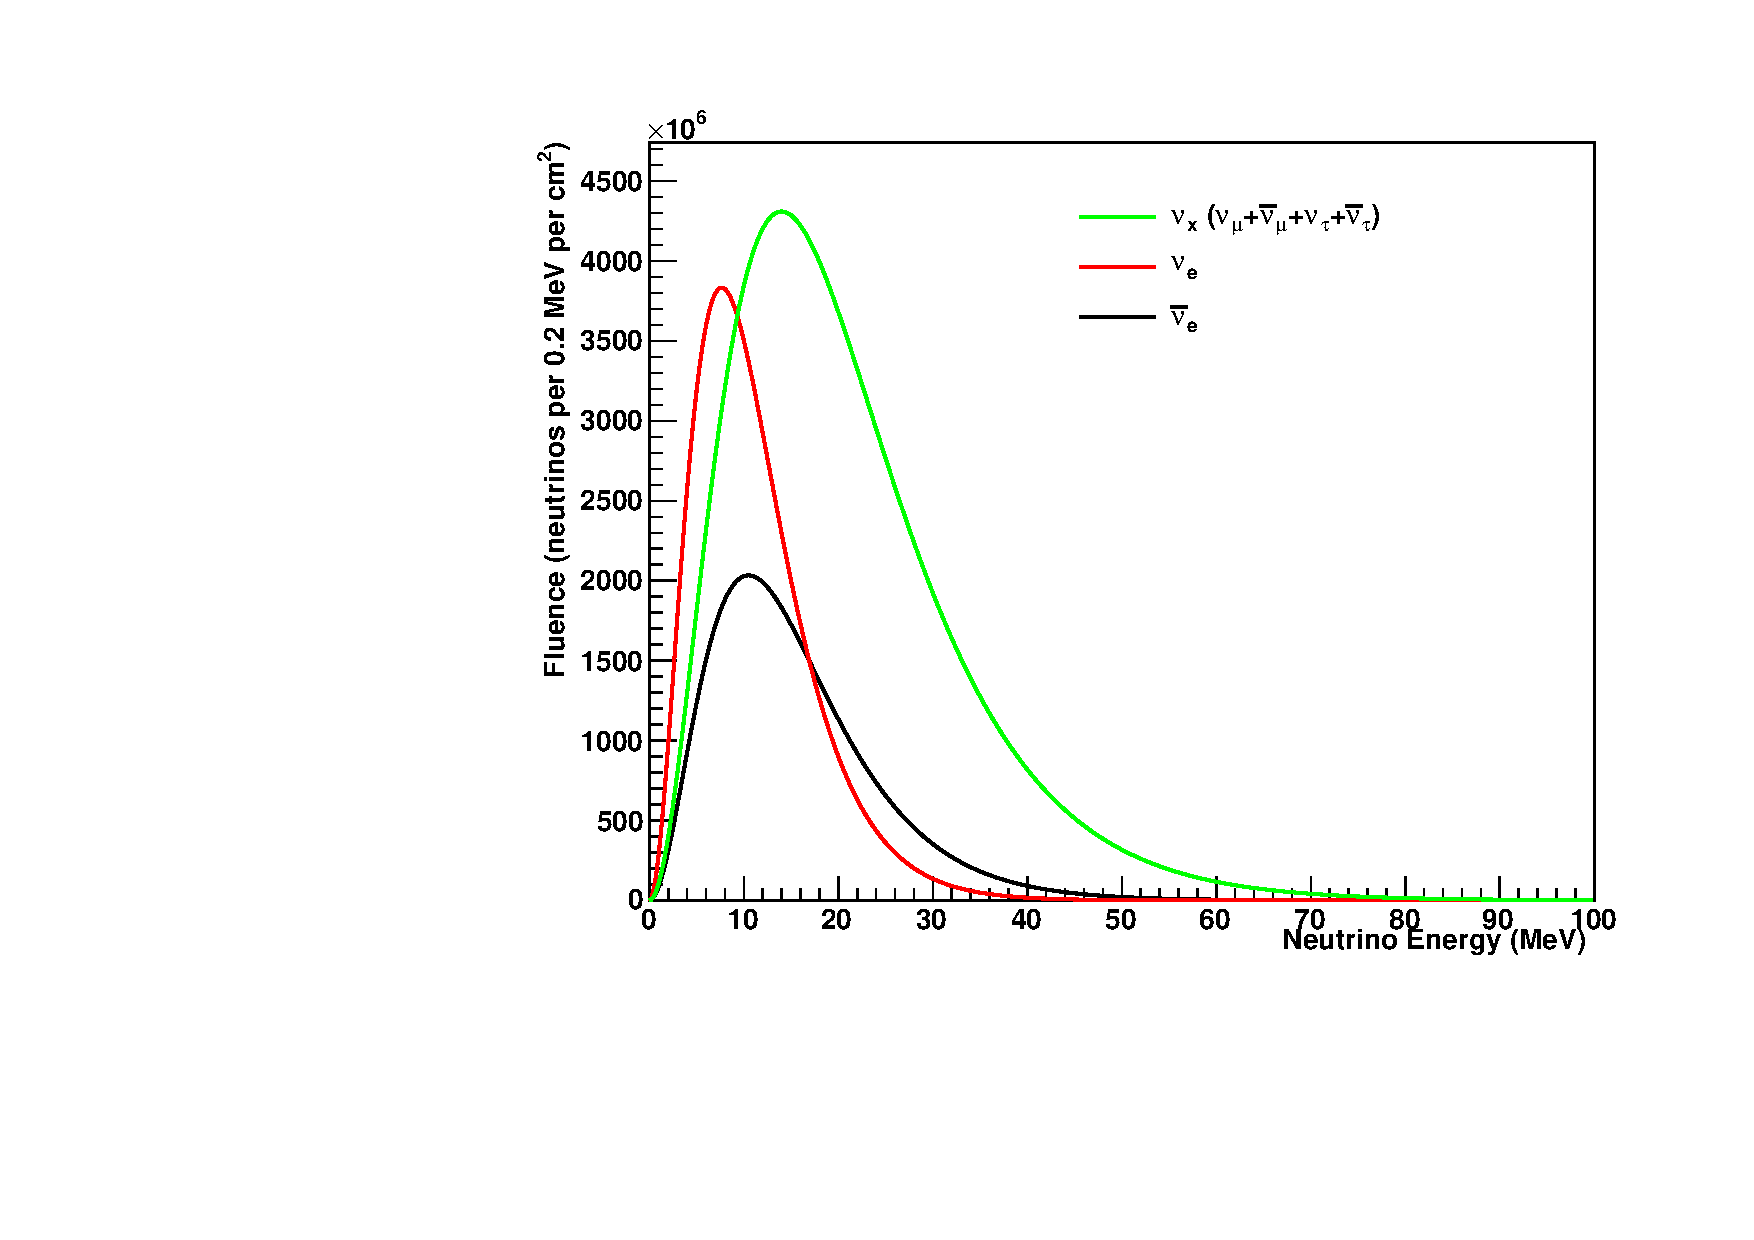
\includegraphics[height=.3\textheight]{figures/flux_livermore.pdf}
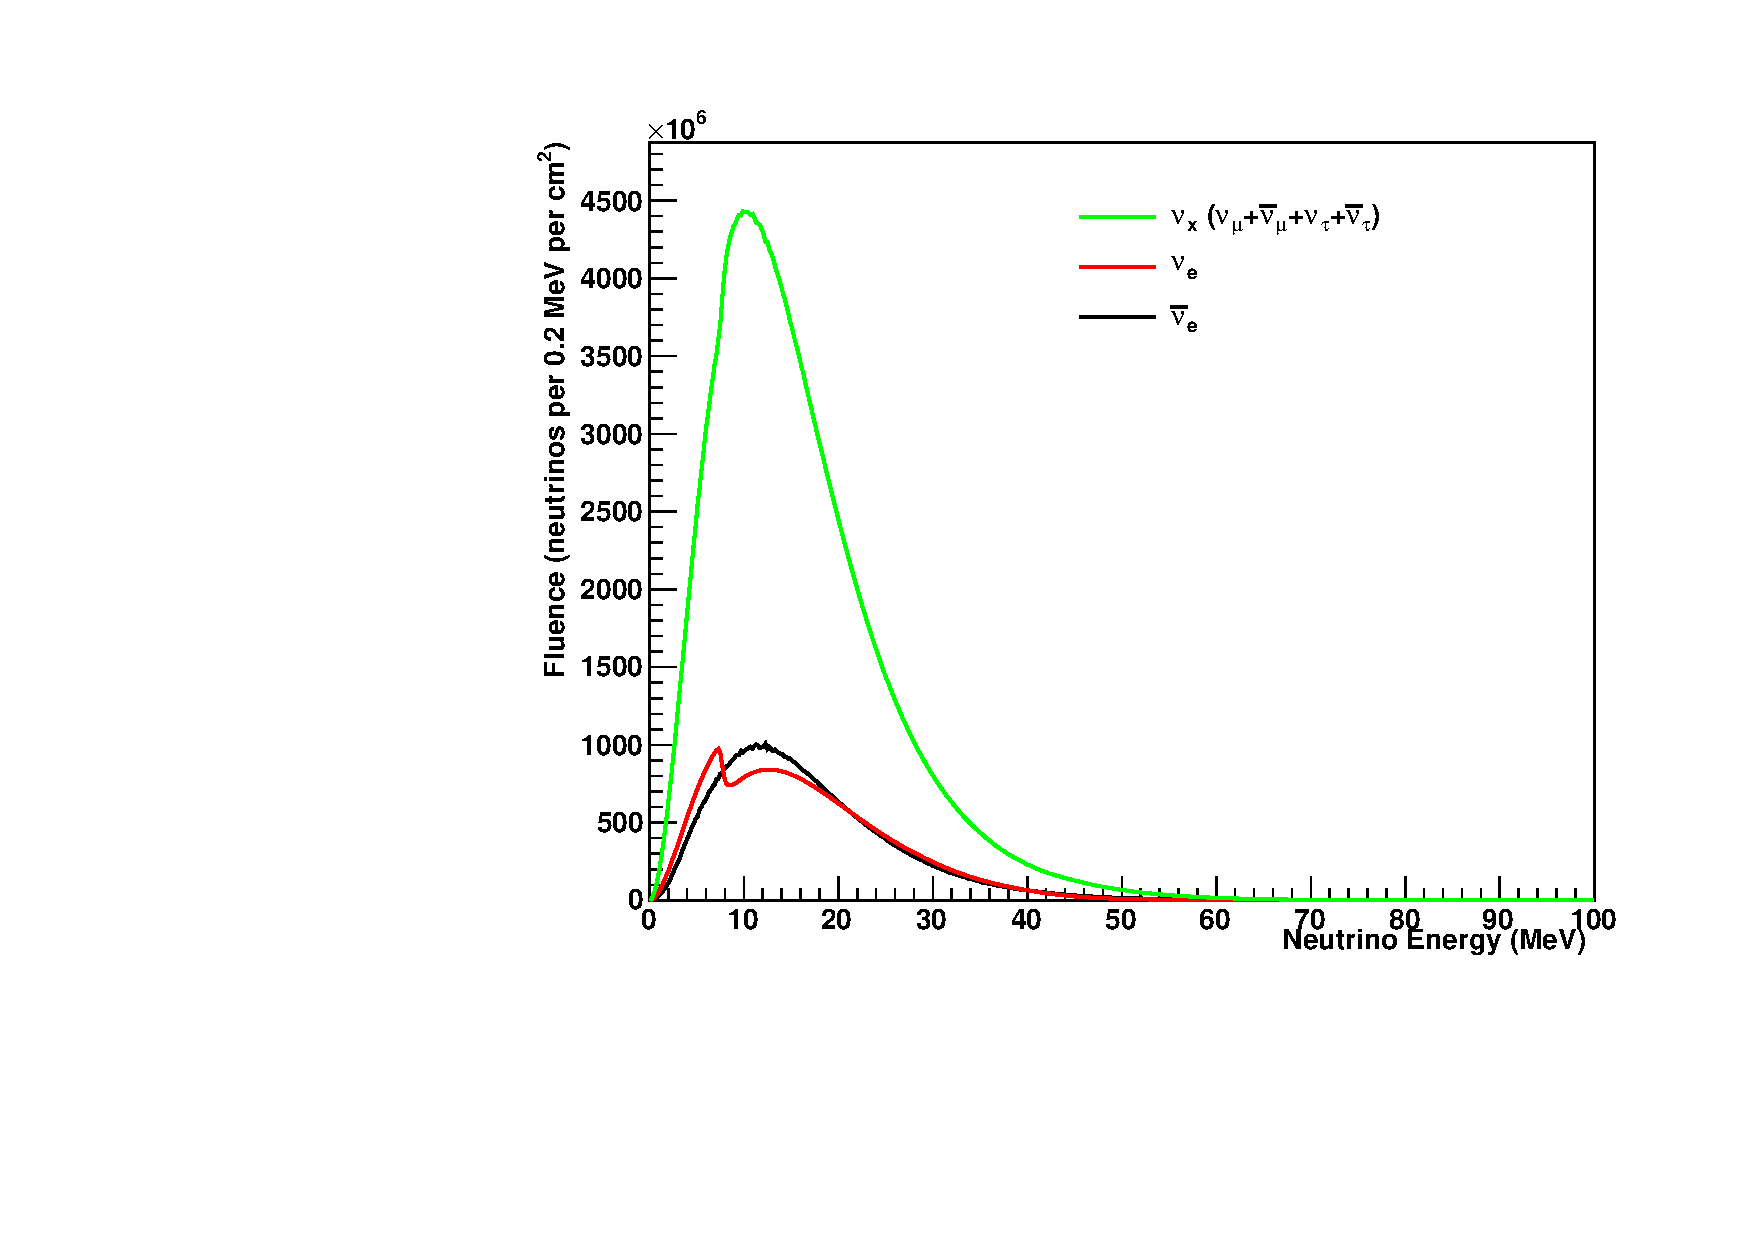
\includegraphics[height=.3\textheight]{figures/flux_gvkm.pdf}

\caption{Left: ``Livermore'' fluence, for different flavor components,
  from reference~\cite{Totani:1997vj}, assuming Fermi-Dirac spectra with
  the average energies indicated as a function of time and zero
  chemical potential, and integrated from $t=0$ to $t=14$~seconds.  Right: ``GVKM'' fluence, integrated over 10
  seconds.}\label{fig:fluxes}
\end{figure}


\section{Neutrino Interaction Cross-sections}

We provide cross-sections relevant for four detector materials relevant for current and near-future detectors:
water, scintillator, argon and lead.  Distributions of interaction
products are taken into account in the ``smearing'' matrices (see Section~\ref{response}).  We
expect future upgrades of $\snowglobes$ to incorporate more channels and
more materials.

\begin{figure}[htb]
  \centering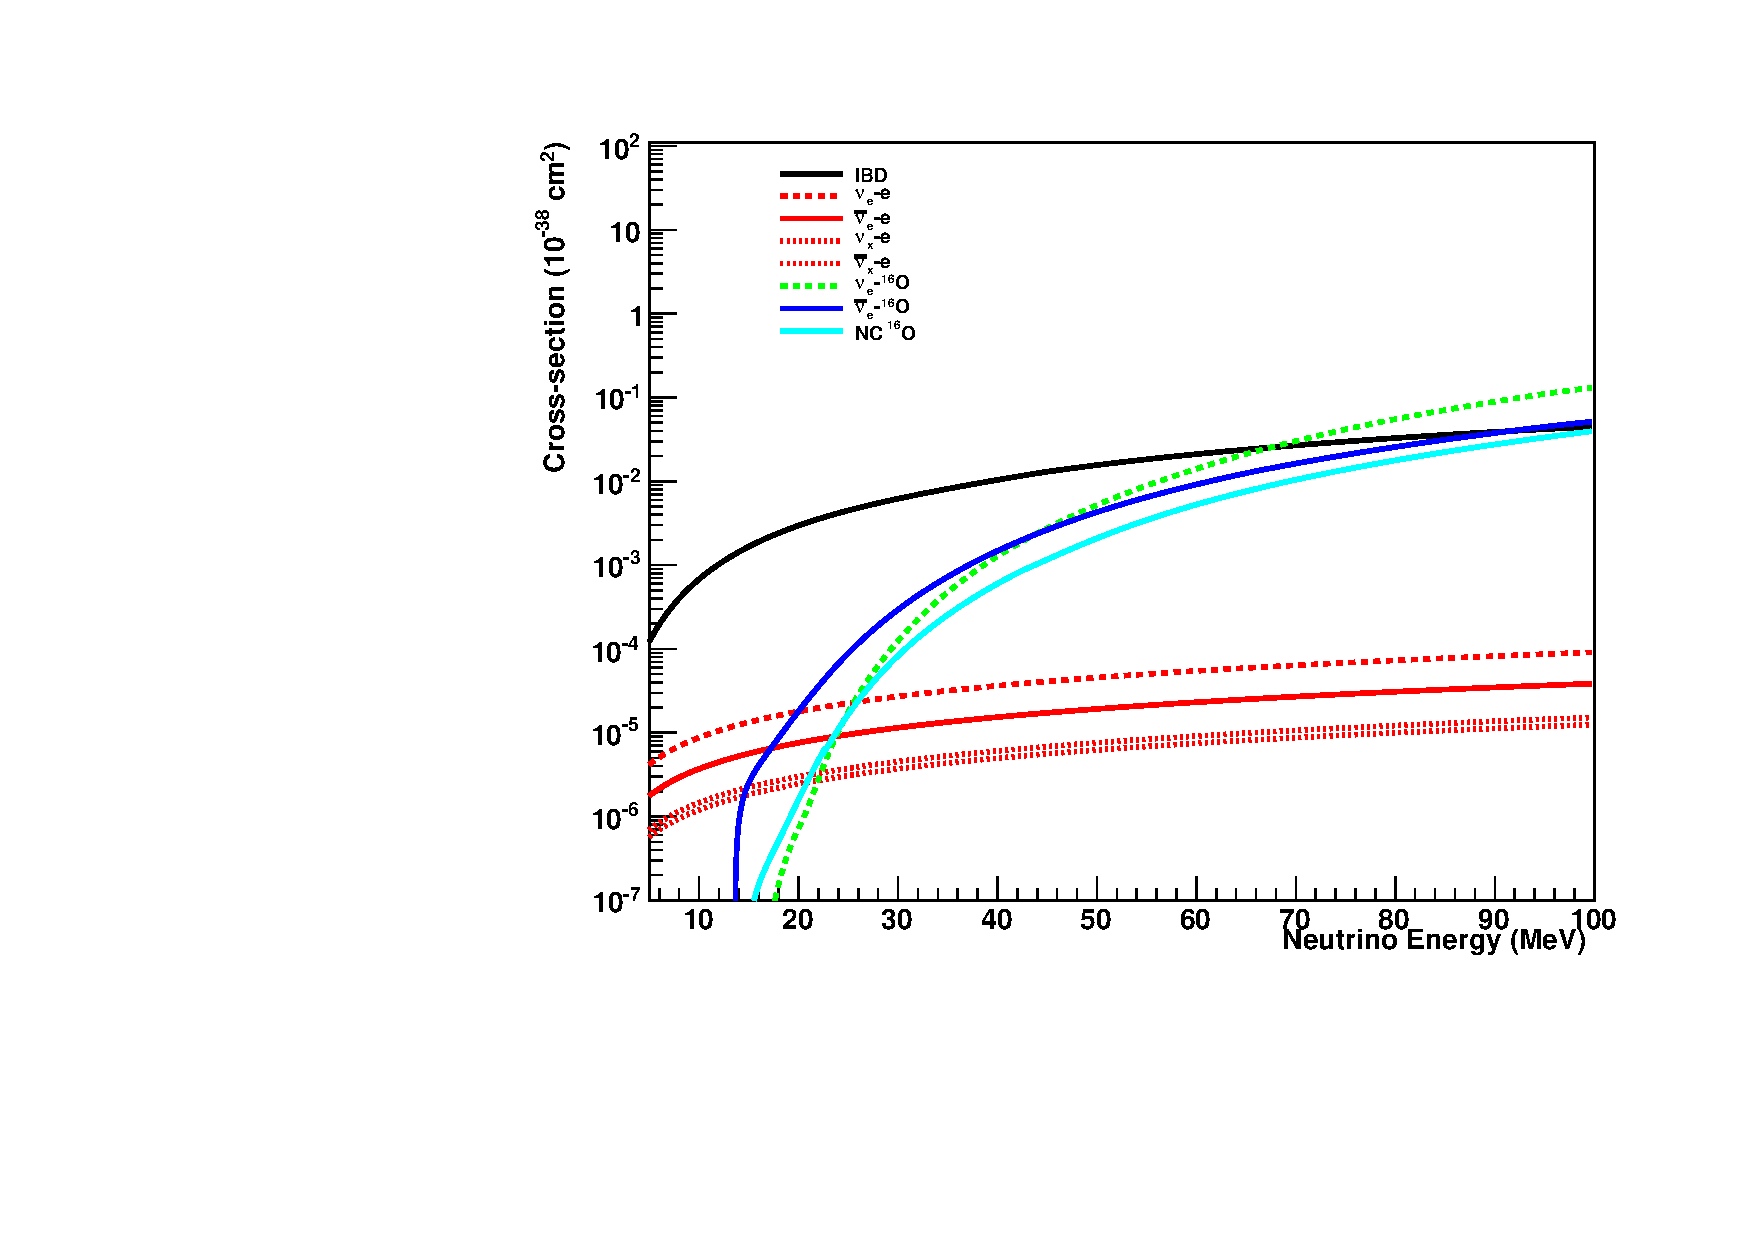
\includegraphics[width=.75\textwidth]{figures/xscns_water.pdf}
  \caption{Cross sections for relevant processes in water.}
  \label{fig:water_xscns}
\end{figure}

\begin{figure}[htb]
  \centering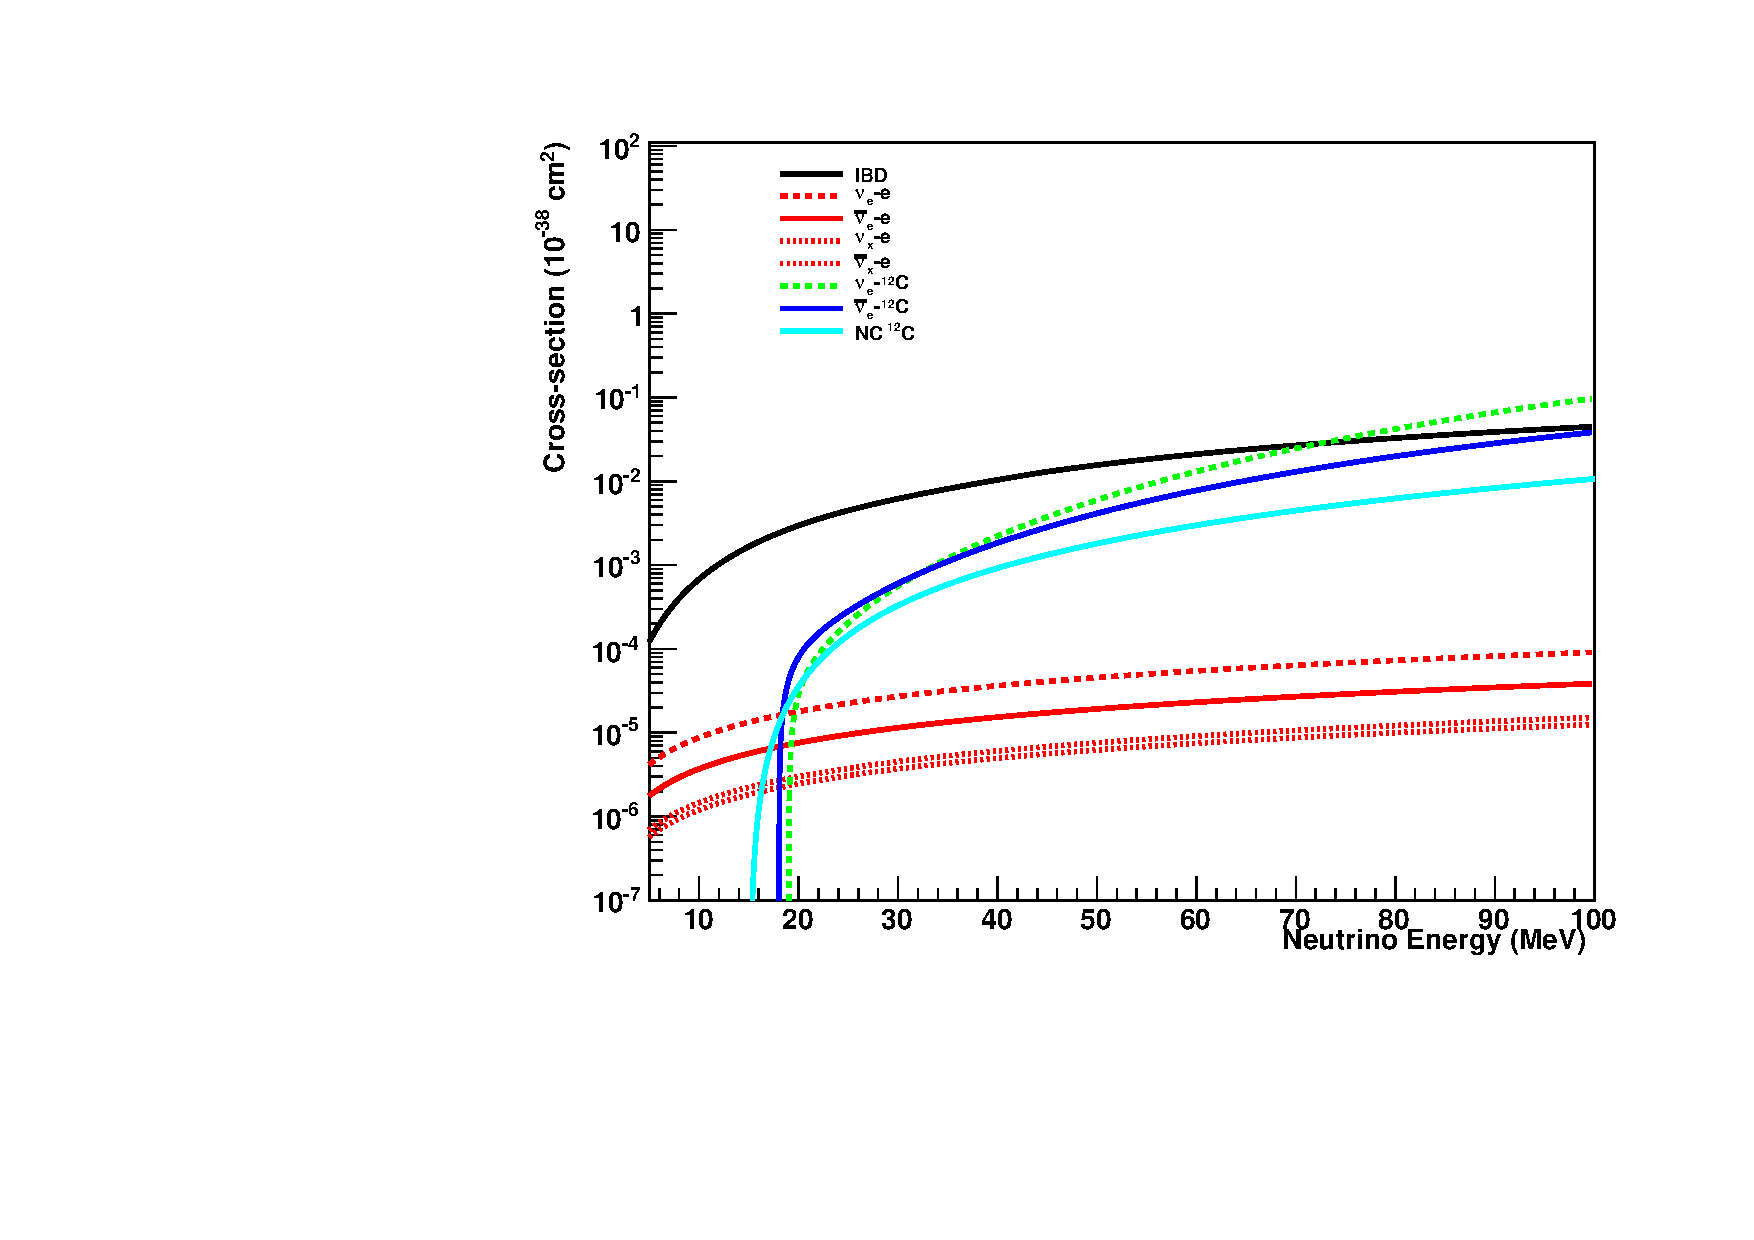
\includegraphics[width=.75\textwidth]{figures/xscns_scint.pdf}
  \caption{Cross sections for relevant processes in scintillator.}
  \label{fig:scint_xscns}
\end{figure}


\begin{figure}[htb]
  \centering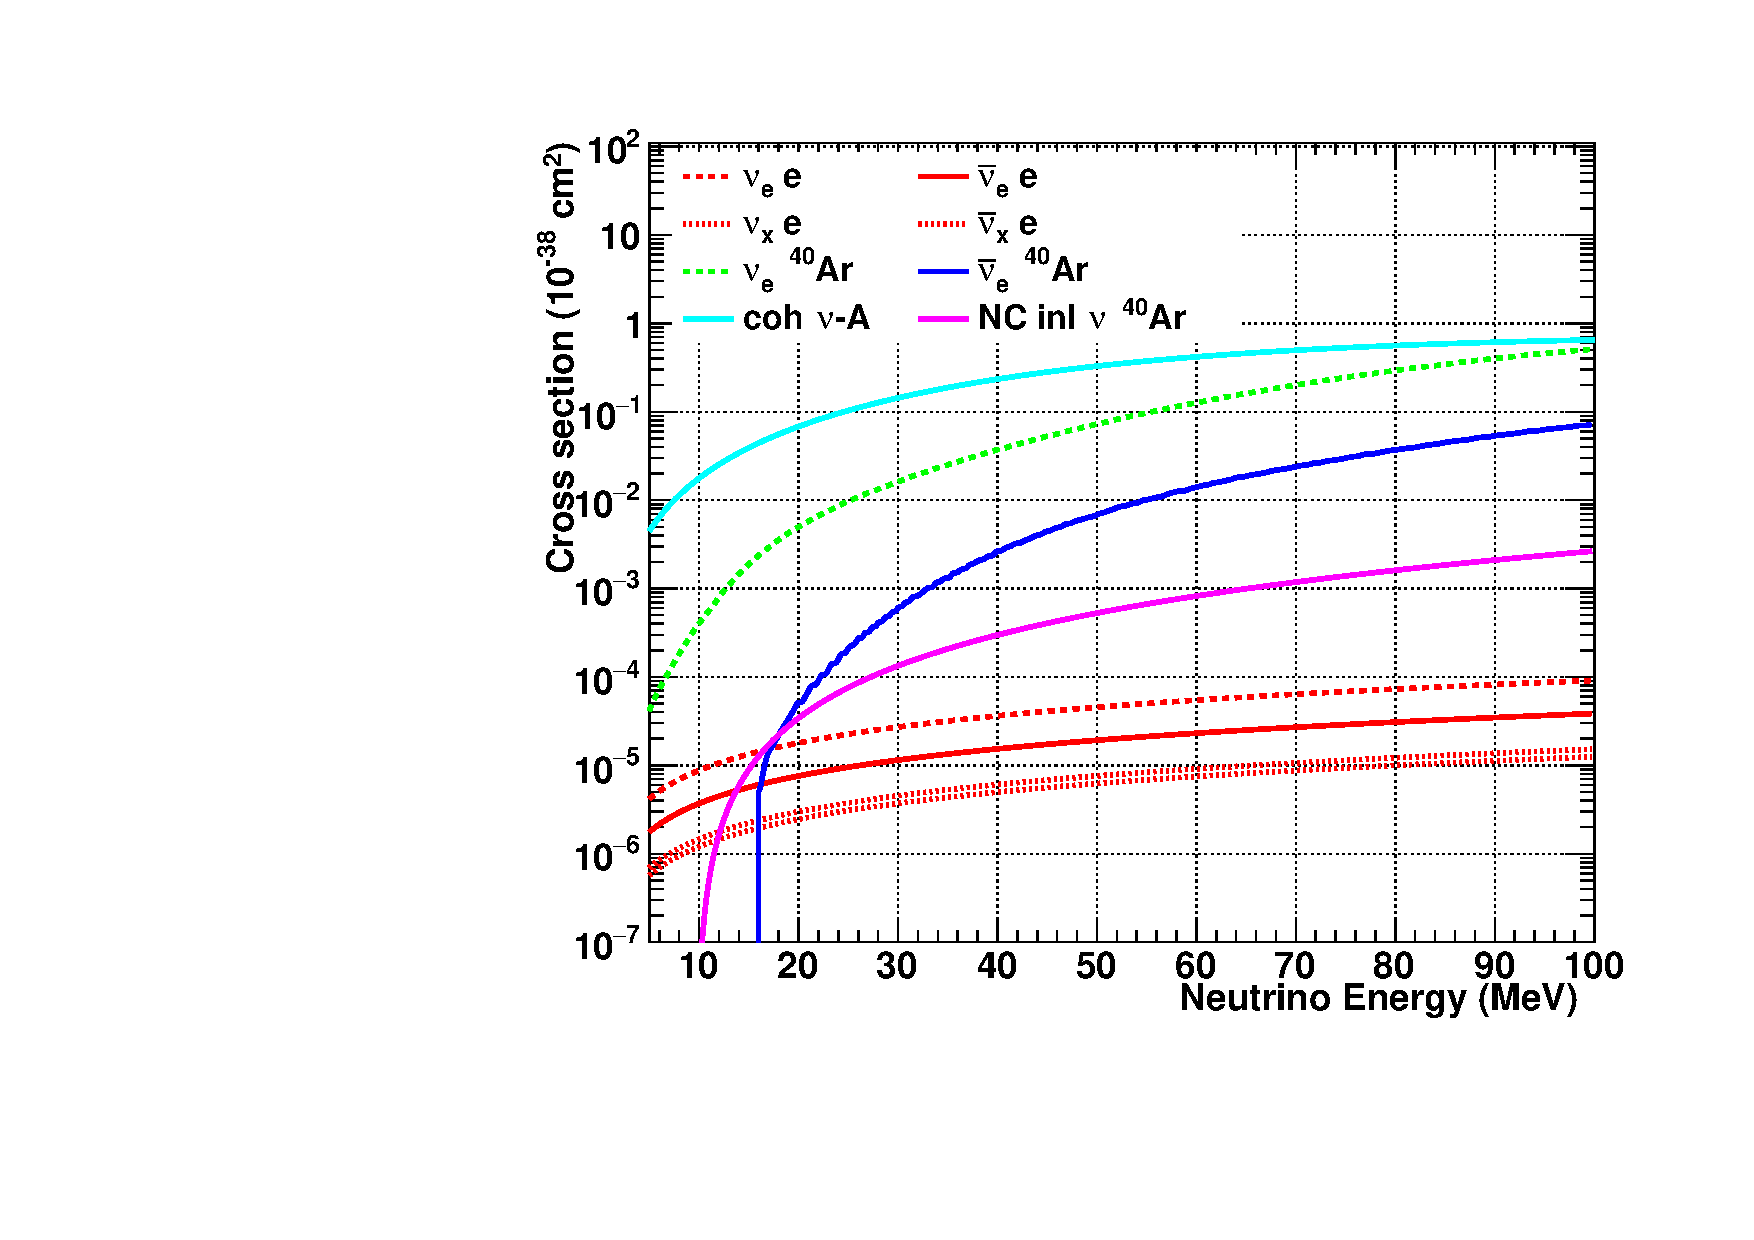
\includegraphics[width=.75\textwidth]{figures/xscns_argon.pdf}
  \caption{Cross sections for relevant processes in liquid argon.}
  \label{fig:argon_xscns}
\end{figure}

\begin{figure}[htb]
  \centering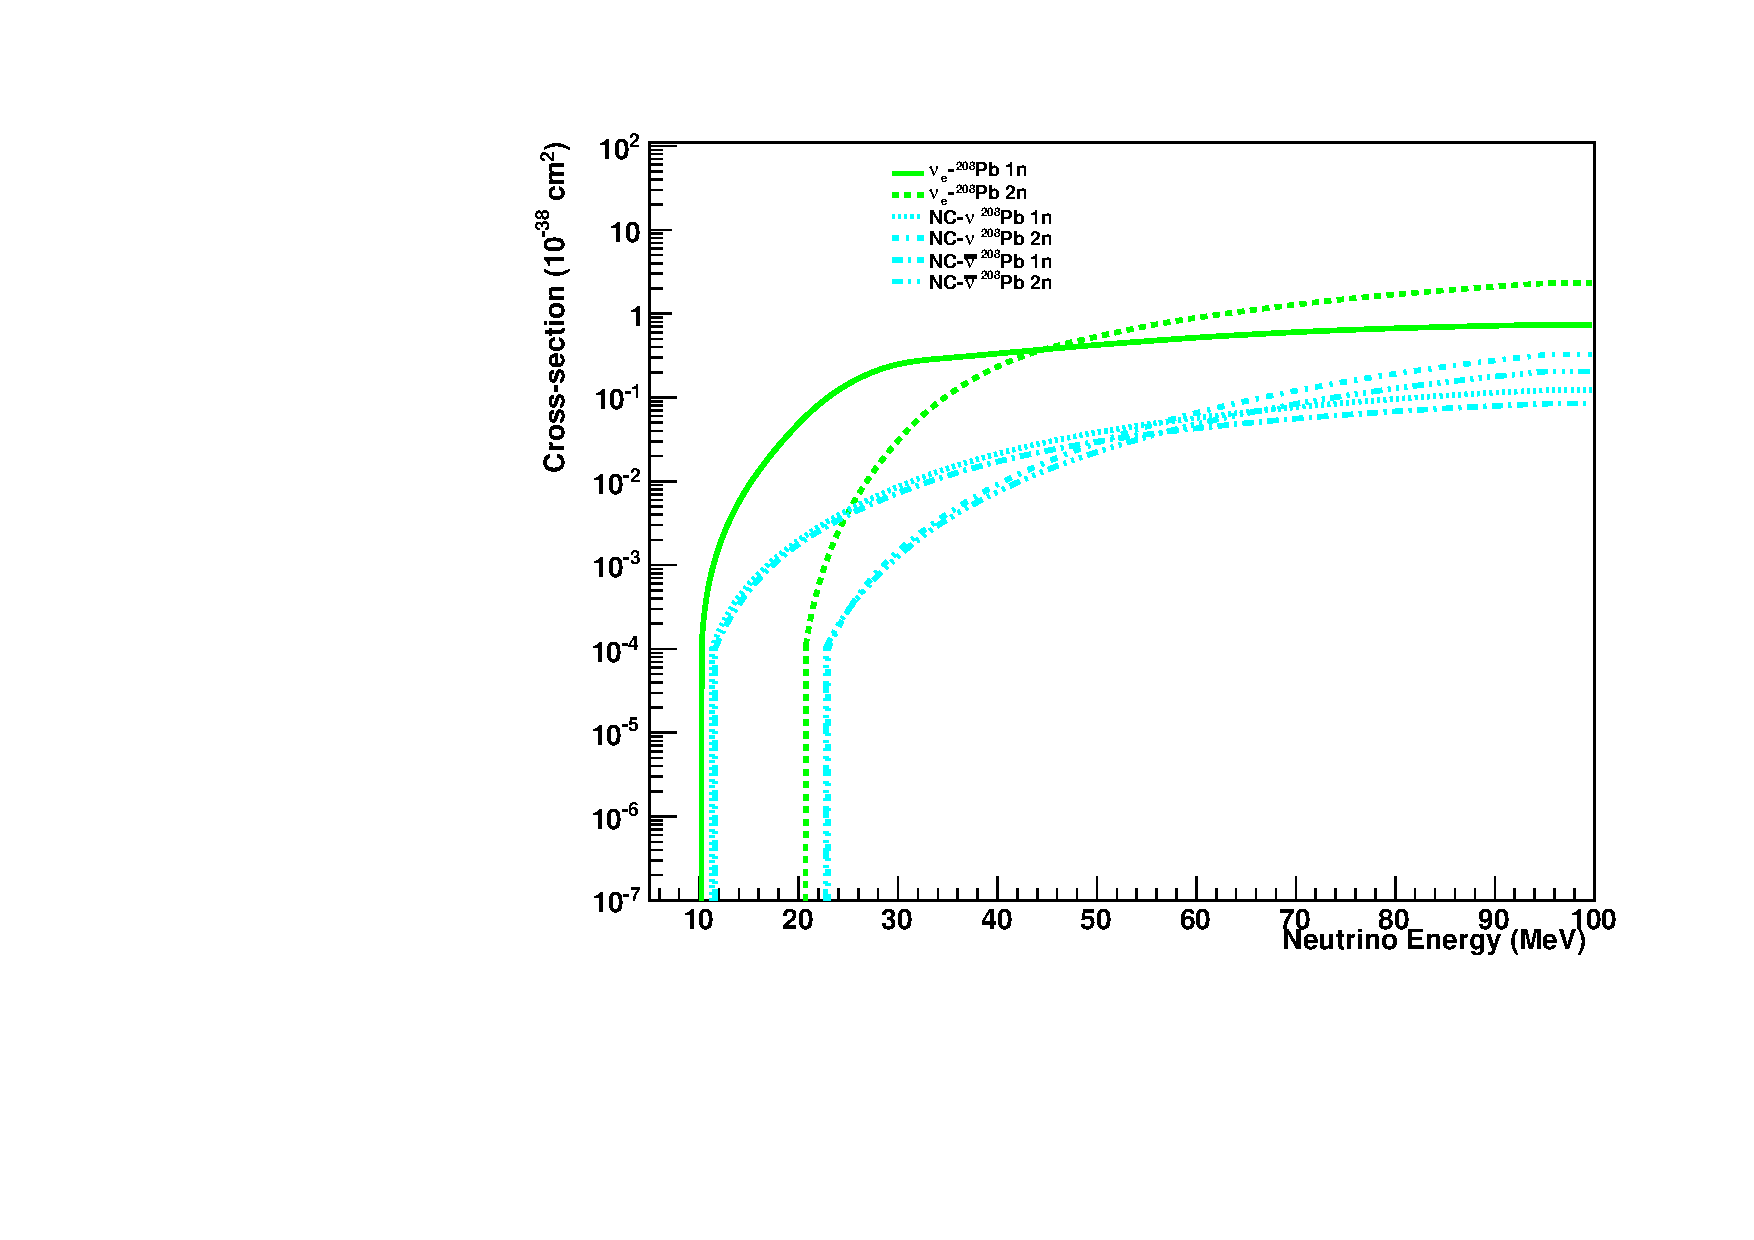
\includegraphics[width=.75\textwidth]{figures/xscns_lead.pdf}
  \caption{Cross sections for relevant processes in lead.}
  \label{fig:lead_xscns}
\end{figure}


\subsection{Inverse Beta Decay}

Inverse beta decay $\bar{\nu}_e+ p \rightarrow e^+ + n$ (IBD) is
dominant for detectors with free protons, such as water and
scintillator.  We use the cross-section from reference~\cite{strumia:2003zx},
plotted in Fig.~\ref{fig:water_xscns}.  


\subsection{Neutrino-Electron Elastic Scattering}

The cross-sections for elastic scattering (ES) of
neutrinos on electrons $\nu_{e,x} + e^- \rightarrow \nu_{e,x} + e^-$
 (both NC and CC) are known to better than percent level~\cite{Marciano:2003eq}.
These cross-sections are plotted in Fig.~\ref{fig:water_xscns}.
The electron ES interaction is relevant for all targets, although the scattered
electrons may not be observable for some detector configurations
(\textit{e.g.} HALO).


\subsection{Interactions with Oxygen}

Interactions on oxygen include the CC interactions $\nu_e+^{16}{\rm
  O}\rightarrow e^-+^{16}{\rm F}$, $\bar{\nu}_e+^{16}{\rm O}
\rightarrow e^++^{16}{\rm N}$.  
These interactions have diverse final states, including
ejected nucleons and deexcitation gammas in addition to the produced
lepton.  For the NC interaction with $^{16}$O, $\nu_x+^{16}{\rm O}
\rightarrow \nu_x+ ^{16}{\rm O}^*$, de-excitation gammas are in principle
observable.  We use cross-sections from reference~\cite{Kolbe:2002gk}.
Oxygen cross-sections are plotted in Fig.~\ref{fig:water_xscns}.

\subsection{Interactions with Carbon}

Electron flavor neutrinos will interact with carbon nuclei via the CC
interactions $\nu_e+^{12}{\rm C}\rightarrow^{12}{\rm N}+e^-$ and
$\bar{\nu}_e +^{12}{\rm C}\rightarrow ^{12}{\rm B}+e^+$. An NC
excitation interaction, $\nu_x+^{12}{\rm C}\rightarrow~\nu_x+^{12}{\rm
  C}^{*}$ also takes place; this interaction results in a 15.5~MeV
de-excitation $\gamma$-ray which can be used to tag this interaction.
We use cross-sections from reference~\cite{Kolbe:1999au} for the CC interactions and the measurement from reference~\cite{Armbruster:1998gk} for the NC cross-section.
Carbon cross-sections are plotted in Fig.~\ref{fig:scint_xscns}.



\subsection{Interactions with Argon}

We include the CC interactions
$\nu_e + ^{40}{\rm Ar} \rightarrow e^- + ^{40}{\rm K^*}$, and
$\bar{\nu}_e + ^{40}{\rm Ar} \rightarrow e^+ + ^{40}{\rm Cl^*}$.
The cross sections for interactions in argon, from references~\cite{GilBotella:2004bv,Kolbe:2003ys},
are shown in Fig.~\ref{fig:argon_xscns}.   The uncertainties for the recent calculations 
are at around the 10-20\% level.
We have recently added the NC inelastic 
$\nu_x + ^{40}{\rm Ar} \rightarrow \nu_x+ ^{40}{\rm Ar}^*$ channel, based on private
communications with Dr. Anna Hayes.  This interaction is assumed to excite the $^{40}{\rm Ar}$
nucleus to the 9.8~MeV level, from which it will de-excite directly to ground, emitting a 9.8~MeV $\gamma$.
The cross sections proved by Dr. Hayes only went up to 52~MeV, so a 2nd order polynomial fit was performed
to the provided cross section curve to extrapolate this up to 100 MeV.  The fit was excellent (save the lowest
energy point, which was manually fixed), so the extrapolation is likely quite valid.


\subsection{Interactions with Lead}

For lead, we include 
CC and NC cross-sections for both single and double
neutron ejection channels for:
$\nu_e + ^{208}{\rm Pb} \rightarrow e^- + ^{208}{\rm Bi}^{*}$, 
$\nu_x + ^{208}{\rm Pb} \rightarrow \nu_x + ^{208}{\rm Pb}^{*}$, 
$\bar{\nu}_x + ^{208}{\rm Pb} \rightarrow \bar{\nu}_x + ^{208}{\rm Pb}^{*}$.

We use cross-sections from~\cite{Engel:2002hg}.
Lead cross-sections are plotted in Fig.~\ref{fig:lead_xscns}.  Uncertainties on lead cross-sections are evaluated in~\cite{Paar:2011pz}.

\section{Detector Response Parameters}\label{response}

The smearing matrices provided are also in $\globes$ format.  The
spectral distributions of interaction products and the detector
response are handled simultaneously by this matrix: each column of the
matrix represents the detector response for a given monochromatic
incoming neutrino energy.  The $\globes$-formatted efficiency files give the
detector efficiency as a function of detected energy for a given channel and detector configuration.  

For some of the provided smearing files, published information was
used; for others, the LBNE simulation package has been used.  Some
estimates may be rather optimistic, as we tend to use optimistic
smearing when little detailed information is available.  Users may
also provide their own smearing matrices and efficiency information.
We will update smearing files as knowledge of
expected detector responses improves.

Background is also handled: the user can provide a file of background as a function of energy to be smeared by the indicated detector response
This is handled by creating a ``fake'' interaction channel and accompanying smearing file.  If a $\globes$-formatted background file labeled by the detector configuration is present in the \texttt{backgrounds} subdirectory, the background will be smeared and an additional output file created.  The user is responsible for 
ensuring that the background events in the file correspond to the same time interval as the signal.

\subsection{Water Cherenkov}

Currently, two water Cherenkov configurations are provided.  The LBNE
detector simulation package, \texttt{WCSim}, was used to create the
smearing and efficiency files for both of these.

\begin{itemize}

\item \texttt{wc100kt30prct}:
This configuration has 100~kton of water with 30\% coverage of high quantum efficiency (HQE) photomultiplier tubes.  Its response is similar to that of Super-Kamiokande I (or III, IV), with 40\% PMT coverage.  

\item \texttt{wc100kt15prct}:
This configuration has 100~kton of water with 15\% coverage of HQE photomultiplier tubes.  Its response is similar to that of Super-Kamiokande II, with 19\% PMT coverage.  


\end{itemize}

For CC channels, we considered only the lepton in the final state,
taking into account the energy threshold.  For the NC interaction we
used a simplified model of the resulting deexcitation gammas by
assuming relative final energy levels according to
reference~\cite{Kolbe:2002gk}.  Because the reference does not provide
differential final state information, we assume the distribution of
these levels is independent of neutrino energy (which is an incorrect
assumption, but probably not a terrible approximation).  The resulting
gamma cascade was simulated using relative probabilities of the
transitions for a given excited state; the resulting gamma spectrum
was then run through the LBNE \texttt{WCsim} detector simulation.  We found rather poor
efficiency for detecting these gammas, in contrast to the results in
reference~\cite{Langanke:1995he}, due to the fact that gammas
frequently scatter electrons below Compton threshold.

Interaction rates and smeared rates for the \texttt{wc100kt30prct} configuration and GVKM model are shown in
Fig.~\ref{fig:wcrates}.  The total rates for each channel (output of \texttt{make\_event\_table.pl}) are shown in Tab.~\ref{tab:wctable}.

\begin{figure}[htb]
  \centering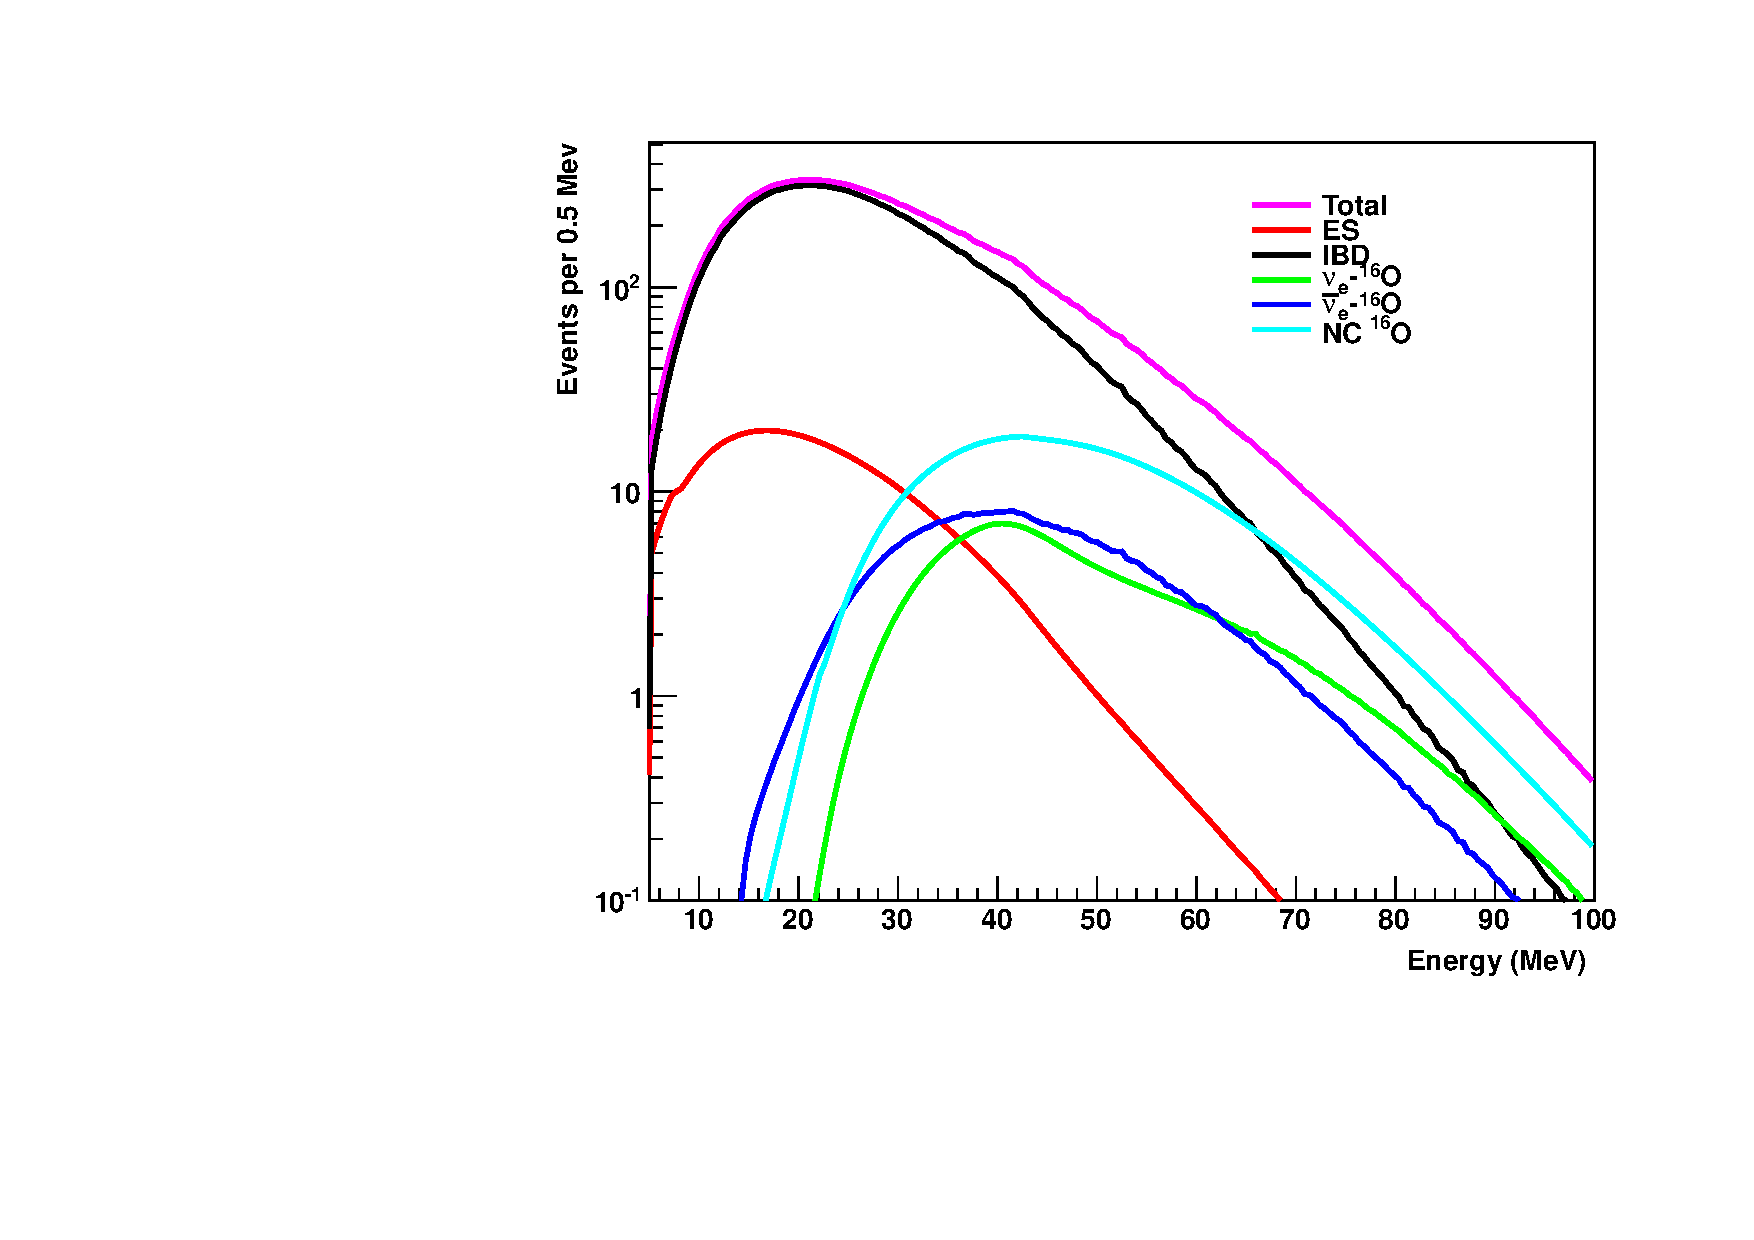
\includegraphics[width=.75\textwidth]{figures/interaction_rates_gvkm_wc100kt30prct.pdf}
  \centering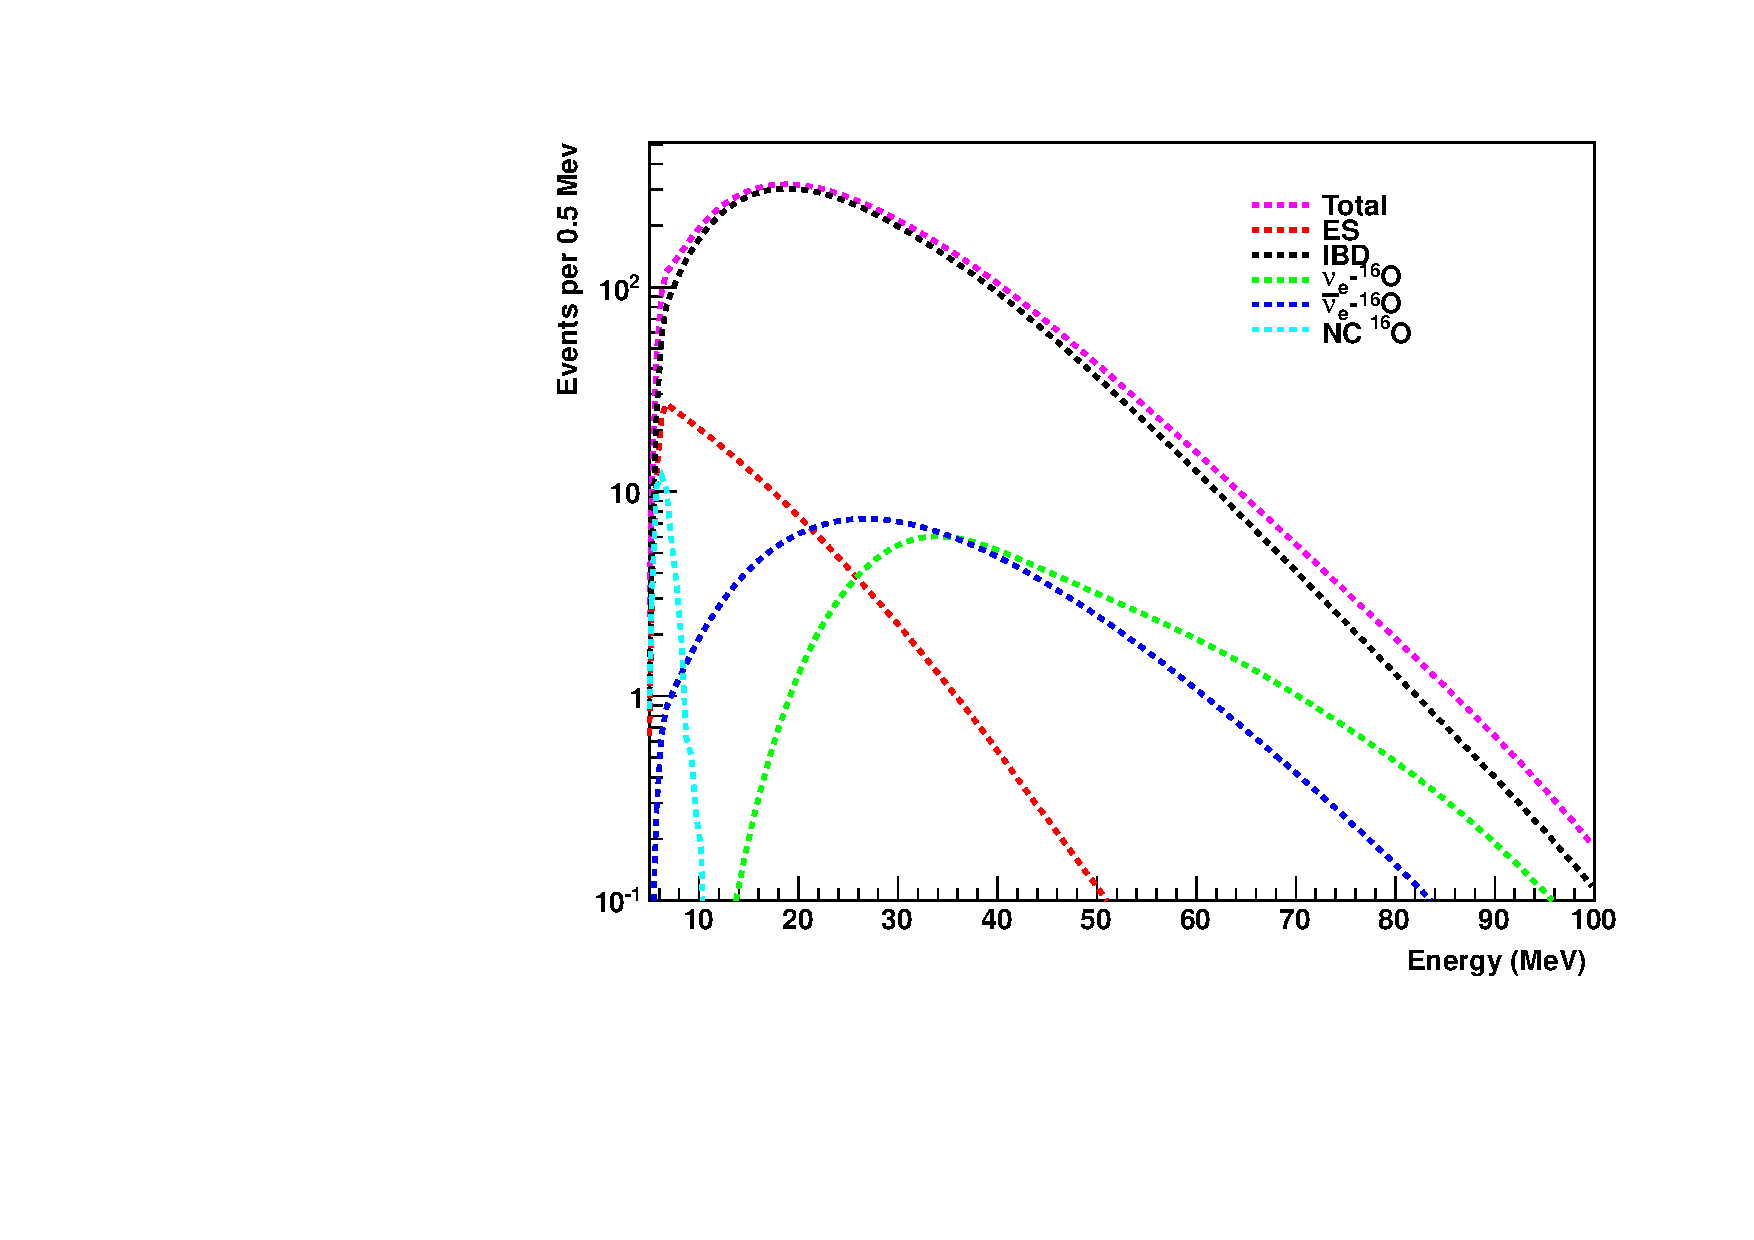
\includegraphics[width=.75\textwidth]{figures/smeared_rates_gvkm_wc100kt30prct.pdf}

  \caption{Event rates in 100~kton of water, for the GVKM model and 30\% PMT
    coverage (events per 0.5~MeV). Top: interaction rates as a
    function of true neutrino energy; bottom:  ``smeared''
    rates as a function of detected energy.}
  \label{fig:wcrates}
\end{figure}

\begin{table}[h]
\centering
\begin{tabular}{|c|c|c|}
\hline
Channel & Events, ``Livermore'' model & Events, ``GKVM'' model  \\
\hline
   $\bar{\nu}_e+ p \rightarrow e^+ + n$                  &  27116 &   16210\\
$\nu_x + e^- \rightarrow \nu_x + e^-$                           & 868 &   534\\
$\nu_e + ^{16}{\rm O} \rightarrow e^- + ^{16}{\rm F}$                         & 88  &  378  \\
$\bar{\nu}_e + ^{16}{\rm O} \rightarrow e^+ + ^{16}{\rm N}$  & 700 &  490 \\


$\nu_x + ^{16}{\rm O} \rightarrow \nu_x+ ^{16}{\rm O}^*$
                         &  513 &  124 \\ \hline
Total &  29284 & 17738 \\ \hline
\end{tabular}
\caption{Total events detected (smeared) for different models in 100~kton of water, for the
\texttt{wc100kt30prct} configuration. }
\label{tab:wctable}
\end{table}

We expect to provide improved smearing and efficiency information for
these and other water Cherenkov detector configurations as the
simulation code development proceeds.

\subsection{Scintillator}

Currently, one scintillator configuration is provided,
\texttt{scint50kt}, representing 50~kton of scintillator.  The
\texttt{scint50kt} smearing files were created using an assumed
resolution of $\frac{\sigma}{E}~=~\frac{7\%}{\sqrt{E {\rm MeV}}}$
from reference~\cite{Eguchi:2002dm}.  At the moment we assume 100\% branching ratio for the 15.1~MeV gamma; however we will refine this in the near future.
Efficiency is assumed to be 100\%.

%\cite{Cadonati:2000kq}

\begin{figure}[htb]
  \centering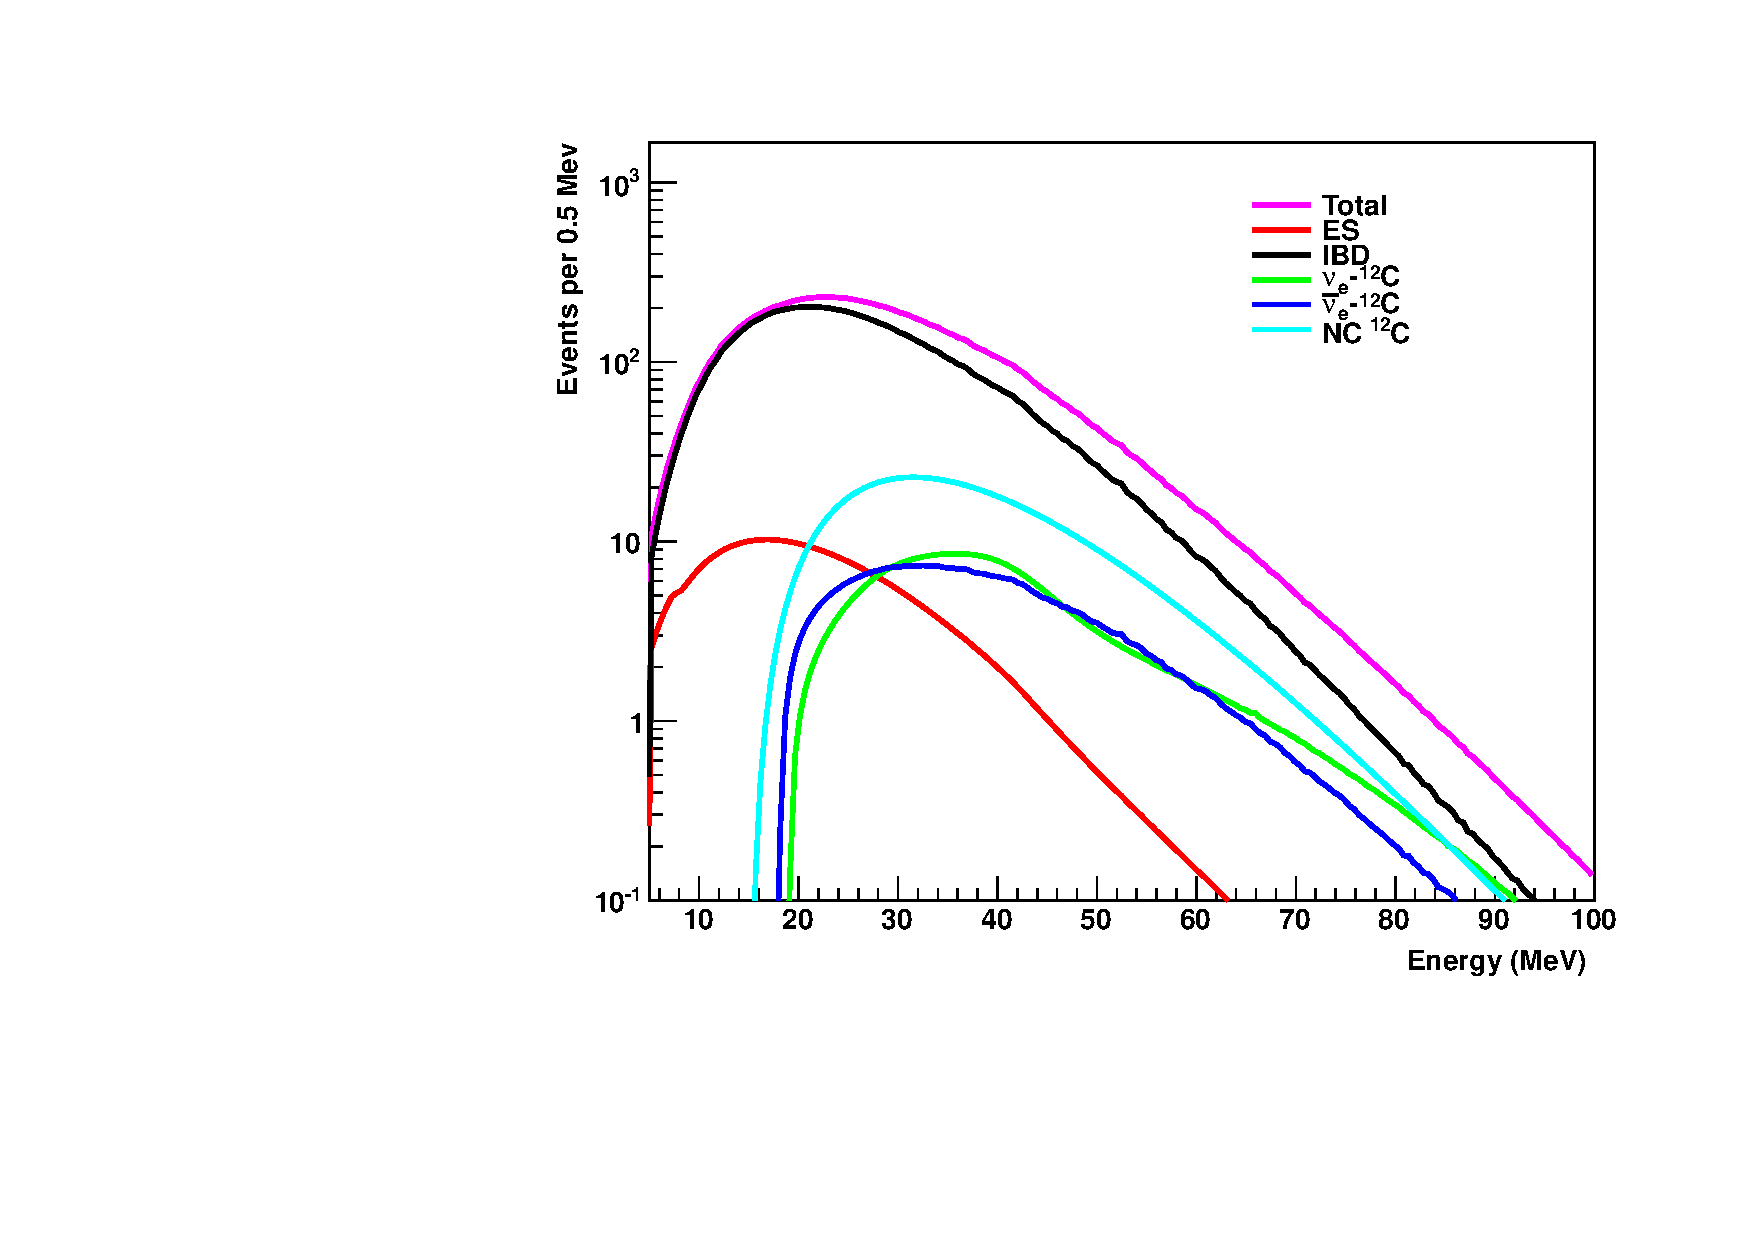
\includegraphics[width=.75\textwidth]{figures/interaction_rates_gvkm_scint50kt.pdf}
  \centering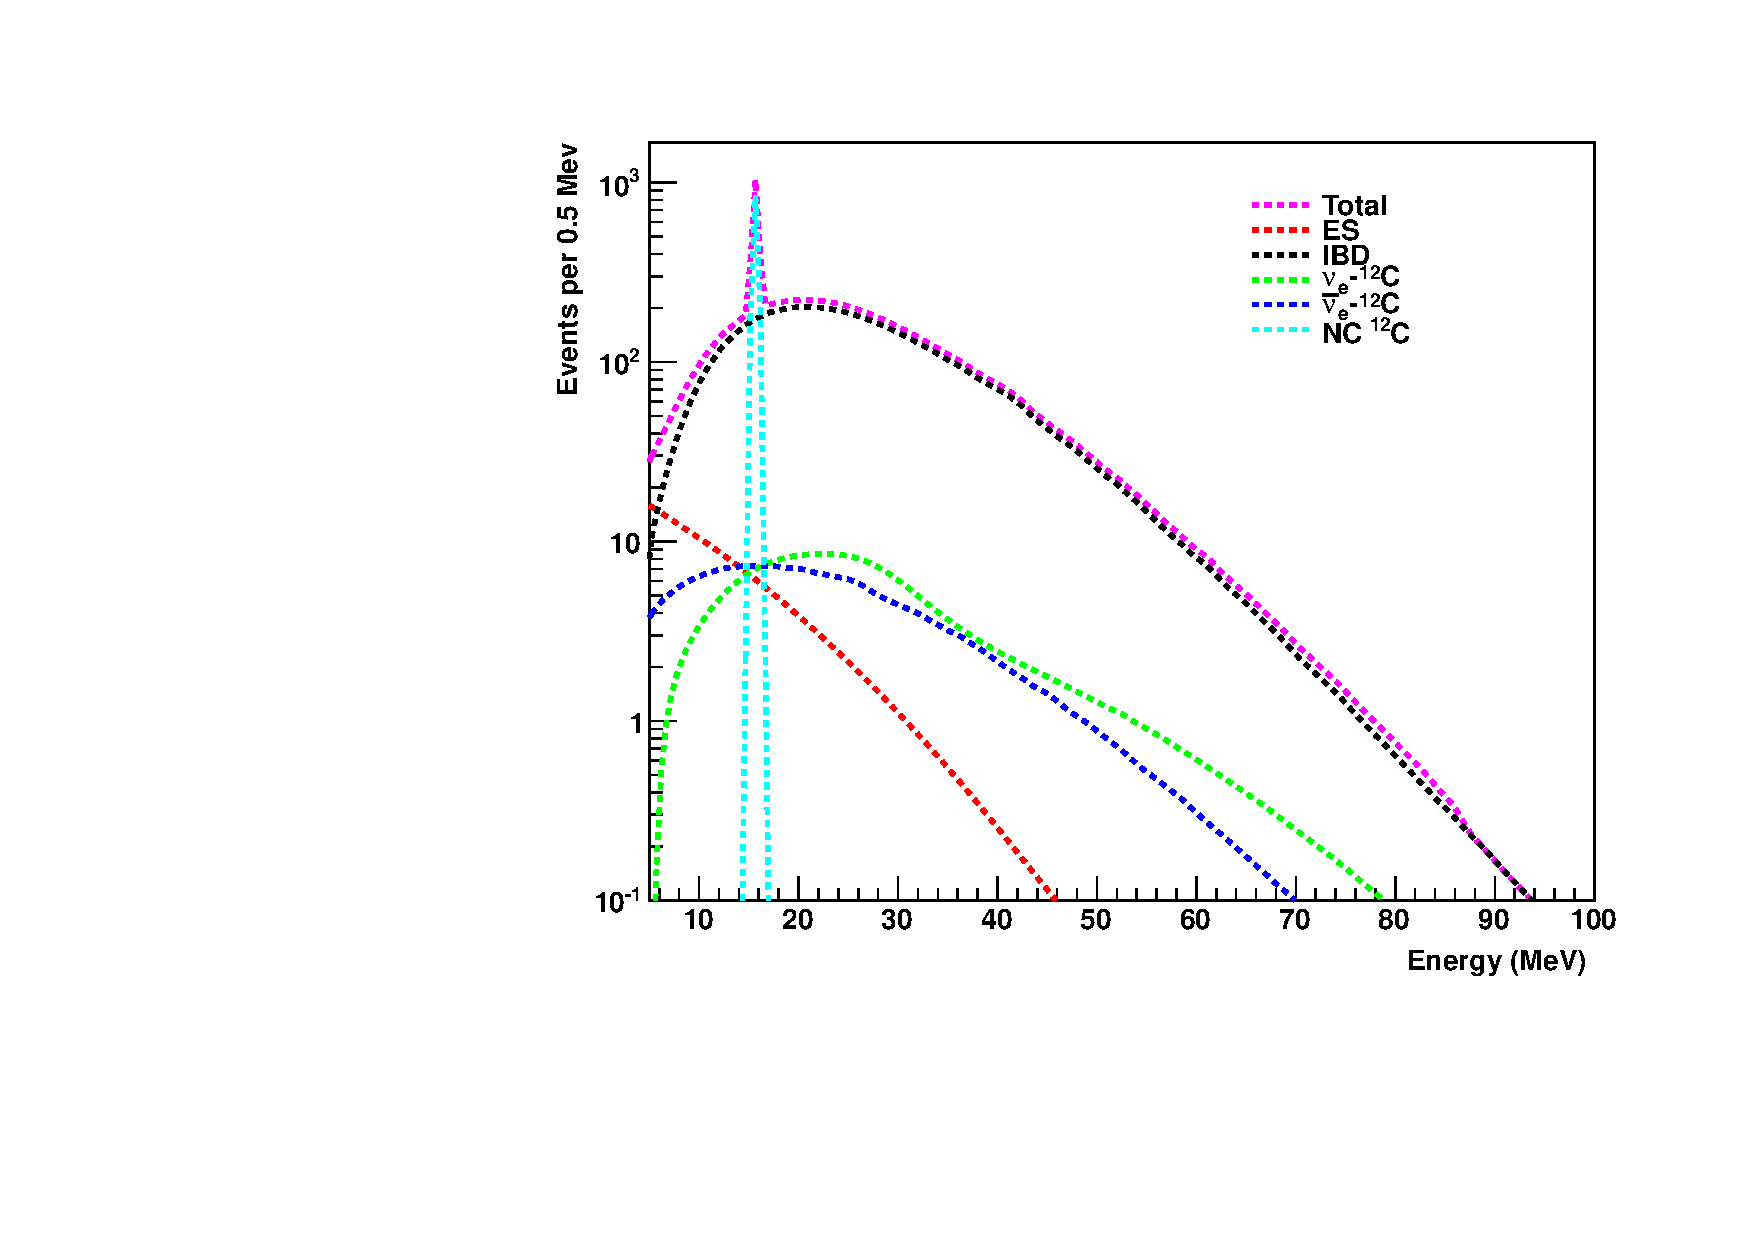
\includegraphics[width=.75\textwidth]{figures/smeared_rates_gvkm_scint50kt.pdf}

  \caption{Event rates in 50 kton of scintillator, for the GVKM model 
  (events per 0.5~MeV). Top: interaction rates as a
    function of true neutrino energy; bottom:  ``smeared''
    rates as a function of detected energy.}
  \label{fig:scintrates}
\end{figure}

\begin{table}[h]
\centering
\begin{tabular}{|c|c|c|}
\hline
Channel & Events, ``Livermore'' model & Events, ``GKVM'' model  \\
\hline
   $\bar{\nu}_e+ p \rightarrow e^+ + n$                  &  17853 &   10617\\
$\nu_x + e^- \rightarrow \nu_x + e^-$                           & 871 &   494\\
$\nu_e + ^{12}{\rm C} \rightarrow e^- + ^{12}{\rm N}$         & 167  &  447  \\
$\bar{\nu}_e + ^{12}{\rm C} \rightarrow e^+ + ^{12}{\rm B}$  & 651 &  439 \\


$\nu_x + ^{12}{\rm C} \rightarrow \nu_x+ ^{12}{\rm C}^*$
                         &  3403 &  1238 \\ \hline
Total &  19601 & 12008 \\ \hline
\end{tabular}
\caption{Total events detected (smeared) for different models in 50~kton of scintillator, for the
\texttt{scint50kt} configuration. }
\label{tab:scinttable}
\end{table}


\subsection{Liquid Argon}

Currently one argon detector configuration is provided,
\texttt{ar17kt}.  For event rate estimates in liquid argon, we assume
a detection threshold of 5~MeV.  We assume also that suitable
triggering will be provided either from charge collection or from some
external trigger.  The energy resolution for the smearing matrices is
from
Ref.~\cite{Amoruso:2003sw},~$\frac{\sigma}{E}~=~\frac{11\%}{\sqrt{E}}~+~2\%$.
For the CC channels in argon we have included energy deposition of the
leading lepton; in the detector response, we also incorporate
additional visible energy from deexcitation gammas (these gammas may
also possibly help to tag the $\nu_e$ or $\bar{\nu}_e$ channels,
in practice).  We assume 100\%
efficiency, for lack of detailed efficiency information available in
the literature.


\begin{figure}[htb]
  \centering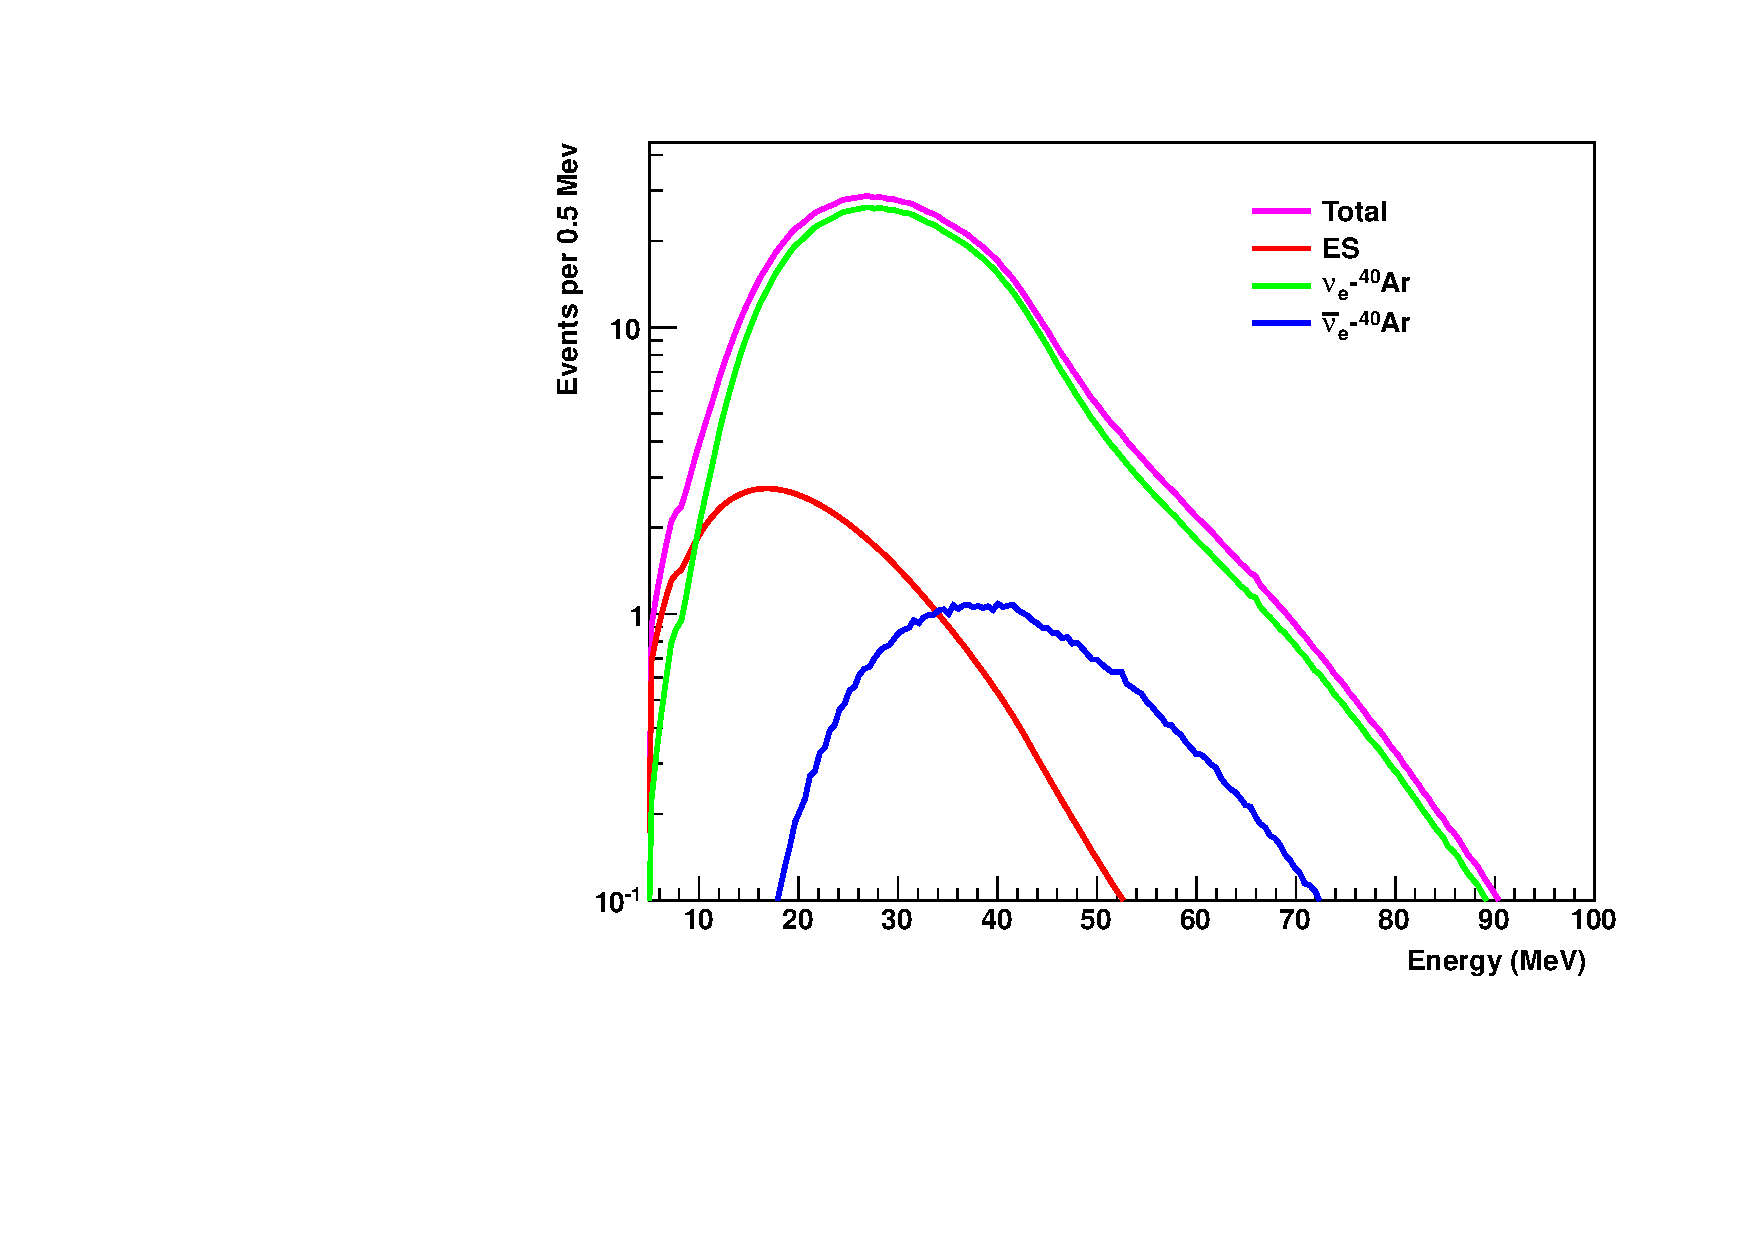
\includegraphics[width=.75\textwidth]{figures/interaction_rates_gvkm_ar17kt.pdf}
  \centering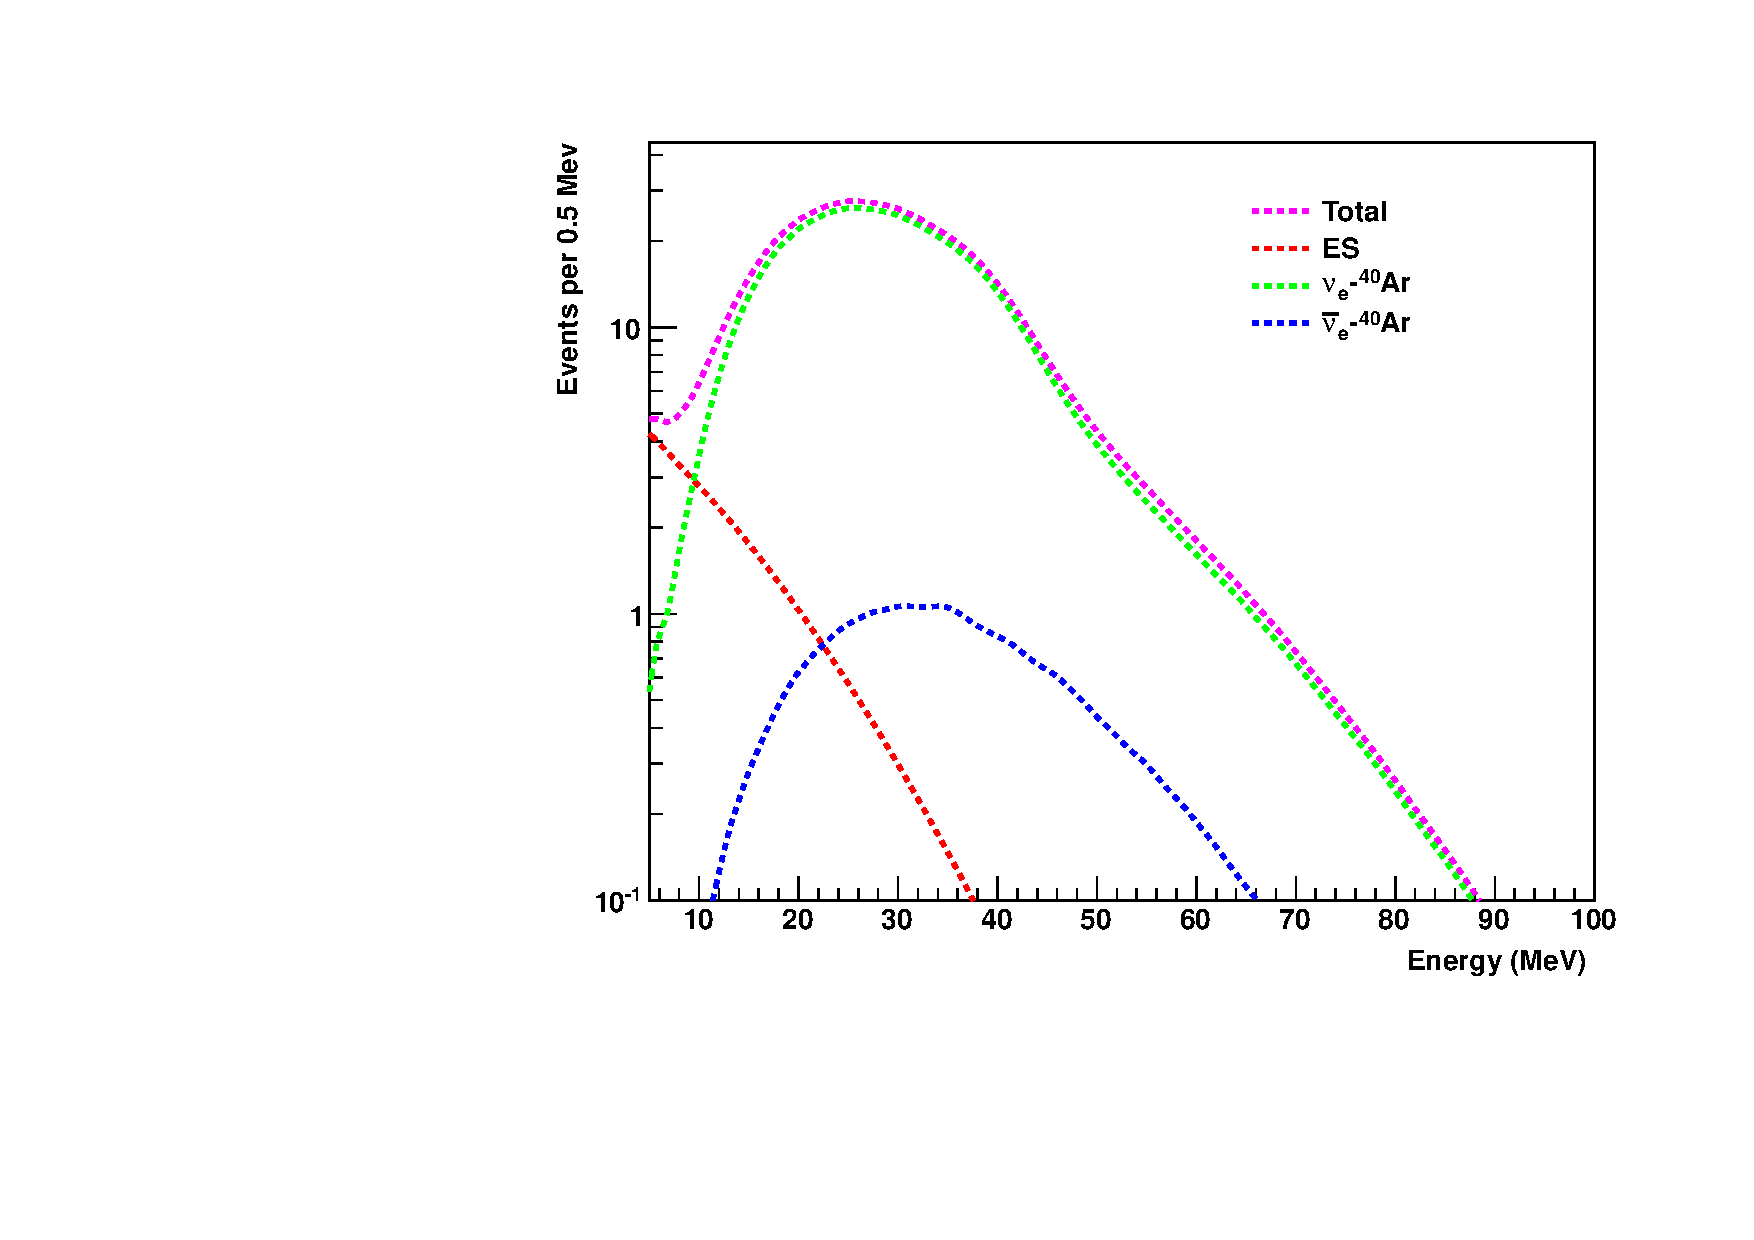
\includegraphics[width=.75\textwidth]{figures/smeared_rates_gvkm_ar17kt.pdf}

  \caption{Event rates in argon, for the GVKM model (events per 0.5~MeV). Top: interaction rates as a
    function of true neutrino energy; bottom:  ``smeared''
    rates as a function of detected energy.}
  \label{fig:larrates}
\end{figure}


\begin{table}[h]
\centering
\begin{tabular}{|c|c|c|} \hline
Channel & Events, ``Livermore'' model & Events, ``GKVM'' model  \\
\hline

$\nu_e + ^{40}{\rm Ar} \rightarrow e^- + ^{40}{\rm K^*}$ & 1138  & 1408 \\

$\bar{\nu}_e + ^{40}{\rm Ar} \rightarrow e^+ + ^{40}{\rm Cl^*}$ & 96& 66\\

$\nu_x + e^- \rightarrow \nu_x + e^-$                           & 146 &   88\\

%$\nu_x + ^{40}{\rm Ar} \rightarrow \nu_x+ ^{40}{\rm Ar}^*$ & & \\ \hline
\hline

Total &  1380 & 1562 \\ \hline
\end{tabular}
\caption{Total events detected (smeared) for different models in 17~kton of argon, in the \texttt{ar17kt} configuration.}
\label{tab:lartable}
\end{table}



\subsection{Lead}

Lead is a special case: for the type of detector configuration under
consideration, HALO~\cite{Duba:2008zz}, electrons are practically invisible
and only neutrons are observable.  In practice, single and double
neutron products from lead can be tagged and reconstructed; although
no event-by-event energy information is available, spectral information can be
inferred from the relative numbers of 1n and 2n events.  The smearing
files in $\snowglobes$ for this configuration are dummy unit matrices;
efficiency of 36\% for 1n channels and 56\% for 2n channels is
applied, although detailed reconstruction efficiencies for true 1n and
2n rates would in practice need to be applied~\cite{halo}.  The user is
advised to make use only of interaction rates for these channels in
lead and to ignore the smeared rates.

\begin{figure}[htb]
  \centering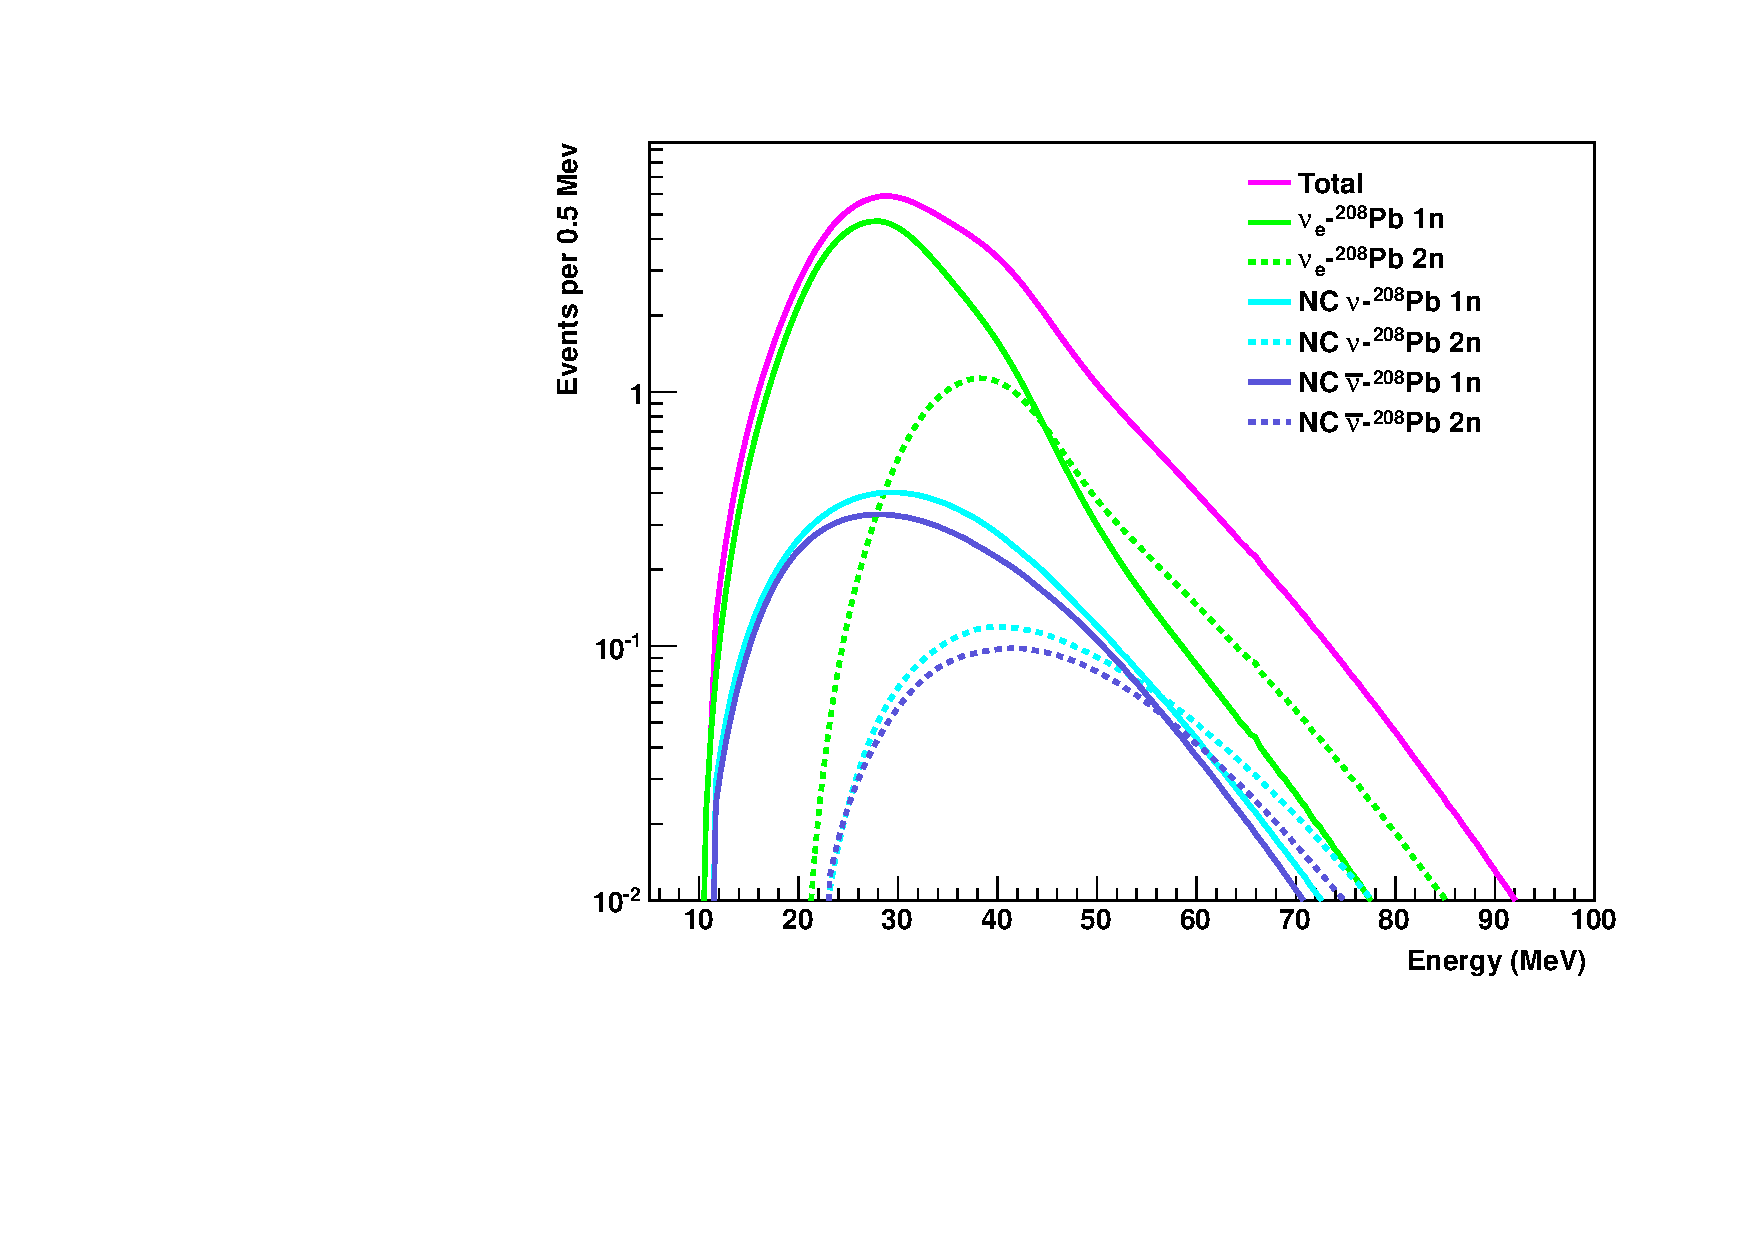
\includegraphics[width=.75\textwidth]{figures/interaction_rates_gvkm_halo2.pdf}
%  \centering\includegraphics[width=.75\textwidth]{smeared_rates_gvkm_halo2.pdf}

  \caption{Event rates in 1~kton of lead (events per 0.5~MeV) for the GVKM model. These
    are interaction rates as a function of true neutrino energy.}
  \label{fig:leadrates}
\end{figure}


\begin{table}[h]
\centering
\begin{tabular}{|c|c|c|} \hline
Channel & Events, ``Livermore'' model & Events, ``GKVM'' model  \\
\hline

$\nu_e + ^{208}{\rm Pb} \rightarrow e^- + ^{207}{\rm Bi} + n$ & 124  &  173\\
$\nu_e + ^{208}{\rm Pb} \rightarrow e^- + ^{206}{\rm Bi} + 2n$ & 14   & 45 \\
$\nu_x + ^{208}{\rm Pb} \rightarrow \nu_x + ^{207}{\rm Pb} + n$ & 53  & 23 \\
$\nu_x + ^{208}{\rm Pb} \rightarrow \nu_x + ^{206}{\rm Pb} + 2n$ & 27  & 7 \\
$\bar{\nu}_x + ^{208}{\rm Pb} \rightarrow \bar{\nu}_x + ^{207}{\rm Pb} + n$ & 48  & 19 \\
$\bar{\nu}_x + ^{208}{\rm Pb} \rightarrow \bar{\nu}_x + ^{206}{\rm Pb} + 2n$ & 23 & 6 \\



\hline

Total & 289  & 272  \\ \hline
\end{tabular}
\caption{Total events detected for different models in 1~kton of lead, in the \texttt{halo2} configuration. }
\label{tab:leadtable}
\end{table}



\section{How to Add Your Own Stuff}\label{addingnew}

It is straightforward to add new fluxes, channels, targets or detector configurations to $\snowglobes$. 

If you add new data files or configurations, the $\snowglobes$ team would appreciate if you would contact us so that the new information can be made available to all users.

\subsection{Adding New Fluxes}

Fluxes can be added by preparing a file according to the
specifications in the $\globes$ manual.  The flux file must be placed
in the \texttt{\$SNOWGLOBES/fluxes} directory and named
\texttt{fluxname.dat}, where \texttt{fluxname} is the chosen name
of the flux.   The file should have 501 rows with flux (or fluence) per 0.2~MeV for the different flavors in each row, for neutrino energies ranging from 0.0001 to 0.1001 GeV.

\subsection{Adding New Channels}\label{addingchannel}
 A new channel for a particular material can be added as a new row in
 the channels file.  Each channel needs a name.  Any text may be used
 to identify the channel, but we use a channel naming convention as
 follows: the channel is \texttt{neutrino\_target}, where \texttt{neutrino}
 is the incoming neutrino flavor 
(\texttt{nue, numu, nutau, nuebar, numubar, nutaubar}).  If the target is a nuclear isotope,
 it's written as the element abbreviation followed by the nuclear $A$,
 \textit{e.g.} \texttt{C12}.  For neutral current (NC) channels, the
 channel name is preceded by \texttt{nc\_} (note that each incoming 
flavor must
 be listed as a separate channel, even though neutral current channels are
 flavor-independent).  Specific exclusive final states, such as
 particular excitations or ejecta, can be denoted with a final tag.
 So for example, the charged current (CC) interaction of $\nu_e$ with
 $^{16}$O is named \texttt{nue\_16O}; the NC
 interaction of  $\bar{\nu}_\mu$ on $^{208}$Pb producing double neutron
 final states is named \texttt{nc\_numubar\_Pb208\_2n}.  (An
 exception to these conventions is inverse beta decay, denoted
 \texttt{ibd}.)

The next item in each channel's row is the channel number; the third
entry indicates whether the incoming neutrino is a neutrino ($+$) or
an antineutrino ($-$); the fourth entry is the flavor of the incoming
neutrino (\texttt{e,m,t}) and the final entry is the target weighting
factor.

The target weighting factor requires a bit more explanation: for each
material, one selects one target ``reference'' type, for which the
weighting factor is unity.  The other targets in the channels file
have target weighting factors indicating the relative number of
targets per reference target.  For example, for water, we have chosen
protons to be the reference target, and inverse beta decay has
weighting factor 1. There are 0.5 $^{16}$O nuclei for each proton, and
5 electrons for each proton in water, so the target weighting factors
for elastic scattering on electrons are 5, and for CC and NC interactions on
oxygen are 0.5.

If you add any new channels to the file, you must provide
cross-sections for these channels and put them in the
\texttt{\$SNOWGLOBES/xscns} directory.  The cross-section files must
be prepared according the the specification in the $\globes$ manual,
and must be named \texttt{xs\_channelname.dat}.  The cross section should be provided between 0.0005 and 0.100 GeV.

\subsection{Adding New Detector Configurations}

The \texttt{detector\_configurations.dat} file contains a list of
available detector configurations.  The first entry in each row is the
detector configuration name.  The second entry is the mass in
kilotons.  The third entry is a target normalization factor: this is
reference targets (see section~\ref{addingchannel}) per
amu in the detector configuration material.  For example,
for water (18 amu per molecule), for which the reference target is protons, the target
normalization factor is $2/18$.  For lead, the reference target is
$^{208}$Pb; the target normalization factor is $1/208$.

Each new detector configuration must have smearing and
(optionally) efficiency files associated with it for each channel the
user wishes to calculate rates for.  The smearing and post-smearing
efficiency files must be prepared according to the specifications in
the $\globes$ manual.  $\snowglobes$ uses 200 true energy bins from 0.0005 to 0.100 GeV and 200 sampling bins over the same range. 
Smearing files must go in the
\texttt{\$SNOWGLOBES/smear} directory and be named as follows:
\texttt{smear\_channelname\_detconfigname.dat}.  Efficiency files must
go in the \texttt{\$SNOWGLOBES/effic} directory and be named as
follows: \texttt{effic\_channelname\_detconfigname.dat}.
If the post-smearing efficiency file is absent, then 100\% post-smearing efficiency is assumed.

\subsection{Adding A New Detector Material}

To add an entirely new detector material, one would create a new
channels file with interaction channels for that material, along with
appropriate cross-section files (and a detector
configuration employing that material).

\subsection{Adding A New Background}

The background calculated by $\snowglobes$ is presumed to be the sum of all relevant backgrounds in the appropriate time interval, as provided by the user.  Backgrounds can be 
be added by creating a file in the \texttt{backgrounds} subdirectory,
\texttt{bg\_chan\_detconfigname.dat}.
If no file is present in this directory for a given detector configuration, $\snowglobes$ will ignore the background.
An accompanying smearing file must be provided by the user,\\
\texttt{\$SNOWGLOBES/smear/smear\_channelname\_detconfigname.dat}.  
If the background is already smeared, this can be the unit matrix.




\section{Future Upgrades}

There are a number of future upgrades on our to-do list:

\begin{itemize}

\item Inclusion of more targets, channels and fluxes.

\item Currently, $\snowglobes$ can handle detected energies in the
  0.5-100~MeV range only.  We plan an upgrade to allow modified output
  energy ranges, which will allow inclusion of channels for which
  the appropriate smeared energy range is different, such as coherent elastic
  scattering on protons or nuclei.

\item As knowledge of detector responses improves (for instance as
  detector simulation codes improve, and measurements are made) we
  will update the smearing matrices accordingly.  

\item Computation of angular distributions for channels with asymmetries.

\item Inclusion of additional cross-sections to allow evaluation of cross-section-related uncertainties.

\item Addition of frameworks for treatment of time-dependent fluxes, and for treating experimental and theoretical uncertainties.

\item Expansion of capability to include multiple, distinct backgrounds.


\item Inclusion of 
   non-supernova fluxes, \textit{e.g.} stopped-pion fluxes.

\end{itemize}

Bug reports, suggestions and contributions are very welcome.  Please
contact Kate Scholberg at \texttt{schol@phy.duke.edu}.


\section{Acknowledgements}

This work was initiated in the context of the Supernova Burst Physics
Topical Group of the Long Baseline Neutrino Experiment collaboration,
for which research activities are primarily supported by the
U.S. Department of Energy and the National Science Foundation.  AB and
NK were supported for work at Duke University by the Deutscher
Akademischer Austausch Dienst summer internship program.  The authors
wish to thank the members of the Physics Working Group of the LBNE
collaboration, and the Institute for Nuclear Theory at the
University of Washington for its
hospitality during the summer of 2010.


\appendix
\section{Change log}

\begin{itemize}
\item Version 1.0 is the initial release.
\item Version 1.1:  the target weighting factors are applied automatically by \texttt{supernova.pl}, which creates correctly-weighted output event rate files from the raw unweighted files (the latter now designated \texttt{\_unweighted.dat}).  Example plotting and event table scripts now no longer apply the weighting factor to event rates, and the user is no longer responsible for doing it.
\item Version 1.2: capacity for handling backgrounds is added; a single background rate per detector configuration is enabled, if provided by the user.  A default background for the \texttt{ar17kt} configuration is included. The NC inelastic interaction cross section is added for $^{40}$Ar.
%cite Vic

 \end{itemize}


\section{GPL}

GPL documentation blurb goes here


\bibliographystyle{unsrt}
\bibliography{refs}


\end{document}
